% siminos/blog/2modes.tex
% $Author: predrag $ $Date: 2012-04-26 23:40:00 -0400 (Thu, 26 Apr 2012) $

% \chapter{Atlas}
% \label{chap:atlas}

\subsection{How to read me}

Here is a novice's guide to desymmetrization bloggery:
\begin{itemize}
  \item
How to read the running blog: go first to the latest blog post, end
of \refsect{chap:atlasBlog}.
  \item
Guys writing the ultimate guide to slicing for the woman on the street,
go to \texttt{siminos/atlas/}, blog in \refchap{chap:atlas}{\em Atlas}.
  \item
If you are reading an article of common interest (which does not fit into
one of the specialized topics), enter your notes into \refsect{chap:atlasBlog}.
  \item
Comments to ChaosBook.org go into ChaosBook.tex section of siminos/blog/.
  \item
Plumbers who ponder how to slice experimental data also blog there,  in
 {\em Symmetry reduction of experimental data}
  \item
Save all figures (pdf or png, not eps) used in the blog in siminos/figs/
sv rm the figures no longer used (they all exist on the repository, if
you need to recover them any time later
  \item
Save useful source programs for figures used in the blog in siminos/figSrc/
  \item
Enter all bibliography items into siminos/bibtex/siminos.bib alphabetically by
first author, create no other *.bib file
  \item
Save useful simulation programs  in (for example) siminos/matlab/
  \item
Never commit large data sets, movies, blog.pdf or anything large that you
can easily recreate.


\end{itemize}

\subsection{How to share literature}
\label{s:HowToLit}

\begin{description}

\item[2012-03-28 PC] \emph{Saved articles.} If you put an article into
Dropbox, I can put it into \HREF{http://ChaosBook.org/library/}
{ChaosBook.org/library}. You can fetch it from there by clicking on
ChaosBook.org/library/BibTexName.pdf (login in as: student Lautrup),
where BibTexName is the name you gave it in siminos/bibtex/siminos.bib.

\item[2012-01-01 PC] In the long run that is a very awkward system, as we
do not have manpower for entering the articles into the
ChaosBook.org/library/index.html, so it is hit and miss finding out
whether a paper you want is there, unless linked it to this blog, like
this:

``Porter and E. Knobloch\rf{PoKno05}
(\HREF{http://ChaosBook.org/library/PoKno05.pdf}{click here})
.''

Much better solution is to join \HREF{http://www.zotero.org/groups/cns}
{www.zotero.org/groups/cns} in order to be able to access the papers we
are saving there, and save your own downloads there of copyright
protected publications. Search for zotero in siminos/blog/blog.pdf to
find a bit more info about it. There you can see what each article is,
use BibTeX to describe it, etc. Ask Gable to help you get started.

\item[2012-03-28 PC]
Put 'our' articles into zotero CNS [library] folder [symmetry] unless the
fit in another section better, enter them into
siminos/bibtex/siminos.bib, and note somewhere in this blog that you have
added them (and why?)

\end{description}



\subsection{Blogging {\twoMode} progress}
\label{chap:2modesBlog}

\begin{description}
\item[2012-04-24 Predrag]
started a new blog, for Chaos Gang term project

\texttt{siminos/cgang/2modes.tex}

\item[2012-03-10 Predrag to Daniel] I put soluChap10.pdf in Dropbox. In
the current edition the programs are renumbered. So far you have done:
\begin{itemize}
  \item[10.8]  An $\SOn{2}$-equivariant flow with two Fourier modes
  \item[10.10] $\SOn{2}$ equivariance of the {\twoMode} system
           for infinitesimal angles.
\end{itemize}
Next bunch of exercises to do:
\begin{itemize}
  \item[10.11] Visualizations of the 5-dimensional {\twoMode} system
  \item[10.22] {\twoMode} system in polar coordinates.
  \item[10.23] The relative equilibria of the {\twoMode} system
  \item[10.24] Plotting the relative equilibria of
           the {\twoMode} system in polar coordinates
  \item[10.25] Plotting the relative equilibria of
           the {\twoMode} system in Cartesian coordinates
\end{itemize}

Still have to make up exercises on group orbits, templates, slicing

%\item[2012-03-21 Daniel]
%Is the {\twoMode} system still of interest or should we put that on the
%back-burner and focus on the \cLe, even if the relative equilibria are
%all circles? I've been writing two versions of every piece of code, one
%for the complex Lorenz system and one for the {\twoMode} system (which is
%still lacking a ``good'' set of parameters that make it nice and
%chaotic). It's not too much work to make one once you have the other, but
%there are details to be addressed, so work would go faster working on a
%single problem.
%
%\item[2012-03-21 Predrag]
%Atlas for \cLe\ is the top priority. The {\twoMode} system is experimental,
%maybe you can get a more interesting system from some truncation of the
%2D Kolmogorov flow. That is totally open.

\item[2012-03-21 Daniel]
From some of the most recent comments copied from pipes/blog suggest that
Rich (I'm assuming Kerswell?) has been looking at periodic orbits in 2D
Kolmogorov flow. Perhaps, the third floor 2D crowd should be in touch
with these guys. Do Mike and Roman know about this?

\item[2012-03-21 Predrag]
Sorry, maybe it is my fault - I just assume everybody tracks the current
literature, I should have told them in person. Here is another relevant
blog entry:

{\bf 2011-05-18  Rich Kerswell} Read Irene Moroz, Geophys. Astrophy Fluid
Dynamics vol 105, 273-286, 2011, \emph{Unstable periodic orbits in 4D
Faraday disk dynamo}. Might give you a 4-dimensional dynamical system
which is chaotic and can be reduced to a 3\dmn\ \statesp; easier to
visualize than {\cLf}.

Kerswell papers are published and easy to find; if you learn something,
please summarize it here for the rest of us.

\item[2012-03-26 Daniel] Looked through various publications by I. Moroz
et al. about a 4D model for a dynamo model that Rich Kerswell had
mentioned as a possible candidate to replace complex Lorenz. This model
has chaotic regimes and some terms that break its discrete symmetries.
There are no continuous symmetries (although don't explicitly say that
they aren't there either), so this might not be a good candidate to
replace complex Lorenz as a toy model for slicing and dicing. However,
the fact that they can find (exact, rather than relative) periodic orbits
probably means that the system does not have continuous symmetries. If it
did it'd be very hard to find exact periodic orbits.
{\bf 2012-03-27 Predrag} I agree, this baby is DOA. Scratch that.

%\item[2007-06-13 Predrag]
%Learned nothing from Armbruster {\em et. al}: they showed that four
%complex Fourier modes suffice to exhibit most of the qualitative features
%of the dynamics, for a wide range of system sizes\rf{AGHks89}.

\item[2009-08-28 Predrag] Evangelos in his thesis and Kohler in his
\HREF{http://ChaosBook.org/projects} {ChaosBook.org project} got nothing
of interest out of Armbruster \etal\rf{AGHks89}.

\item[2012-03-26 Predrag]
There is Armbruster, Guckenheimer and Holmes\rf{AGHO288} flow with
$\On{2}$ symmetry:
\index{Armbruster-Guckenheimer-Holmes flow}
\beq
\begin{split}
  \dot{z}_1 &=\bar{z}_1 z_2
              + z_1\left(\mu_1+ e_{11}|z_1|^2+e_{12}|z_2|^2\right) \\
  \dot{z}_2 &=\pm z_1^2
              + z_2\left(\mu_2+ e_{21}|z_1|^2+e_{22}|z_2|^2\right)
  \label{eq:AGH}
\end{split}
\eeq
where $z_1,z_2\in \mathbf{C}$ and $\mu_j$ and $e_{jk}$ real parameters.
This system corresponds to the first few terms in the center manifold
reduction of a $\On{2}$-symmetric partial differential equation near a
codimension two bifurcation. It is a {\twoMode} system, so group orbits are
more interesting than for \cLf.
{\bf [2009-08-28 Predrag]} Evangelos in his thesis and
\HREF{http://chaosbook.org/projects/index.shtml\#Kohler}{Kohler} in his
\HREF{http://ChaosBook.org/projects}
     {ChaosBook.org project}
got nothing of interest out of Armbruster \etal\rf{AGHO288}. As far as we
can tell, it exhibits no chaos. I would prefer some modification of it
with $\SOn{2}$ symmetry only, and exhibiting chaos (done! see 2012-03-27
remark below). Or some version of {\twoMode} model Daniel has been playing
with which does not behave singularly. He has an unstable cycle close to
the origin that maybe does the trick.


\item[2012-03-26 Daniel] \refRef{PoKno05} and two others may provide some
candidate systems. Haven't had time to enter them into siminos.bib or
read through them but the look promising.

\item[2012-03-27 Predrag to Keith]
{\twoMode}\rf{PoKno05}
(\HREF{http://ChaosBook.org/library/PoKno05.pdf}{click here})
write: ``Chossat\rf{Choss93} has shown that breaking the symmetry
$\On{2}$ down to $\SOn{2}$ through the addition of small terms that break
reflection symmetry generically destroys the heteroclinic cycles and
replaces them by a quasiperiodic orbit characterized by two small
frequencies, one associated with the broken heteroclinic connection and
one with a slow drift along the group orbit of translations. Ashwin
\etal\rf{AshBoMe96} showed that this perturbation must be dispersive: if
reflection symmetry is broken by adding a constant through flow the cycle
will persist.''

This shows us how to get an $\SOn{2}$-equivariant model rather than
the Armbruster, Guckenheimer and Holmes\rf{AGHO288}:
``When the reflection symmetry is broken, the coefficients in the normal
form equations are no longer forced to be real and hence can be expected
to acquire imaginary parts'', their Eq. (10). Play with that one.

\item[2012-03-28 Daniel]
Rodriguez and Schell\rf{Rodriguez1990} may actually be a good system.
They are using a truncation of the Ginsberg-Landau equation, which
results in a 4D system of ODE's. These equations have parameters regimes
that are chaotic (as reported by Rodriguez and Schell and at least one
other researcher). They are $\SOn{2}$-equivariant. They only have a small
number of parameters (3). The truncation is a two-mode truncation so it
should provide more interesting group orbits than the one-mode Complex
Lorenz system.

``Within the two-mode approximation, and using
the transformation
\[ a_k = (b_k, c_k) = b_k + ic_k = r_k e^{i\theta_k}\,, \]
the LG equation reduces to a set of four ordinary differential equations
for the variables $r_0$, $r_1$, $\theta_0$, $\theta_1$; however, it is
more convenient to replace the last two variables with the linear
combinations $\psi_1 = \theta_1 -\theta_0$, which is a phase difference,
and $\zeta = \theta_1 +\theta_0$, which is a phase sum.
''

\end{description}
Their system of equations is:
\index{Rodriguez and Schell flow}
\beq
\begin{split}
  \dot{r}_o &= \rho r_0\left( 1 - r_o^2\right)
                - r_0 r_1^2\left(\rho + \frac{1}{2}\rho\,\cos(2 \pi \psi_1)
                + \frac{1}{2} \sin(2 \pi \psi_1)\right) \\
  \dot{r}_1 &= (\rho - q^2 c_0)r_1 - \frac{3}{4}r_1^3 - r_1 r_0^2 \left(2 \rho
               + \rho\,\cos(2 \pi \psi_1) - \sin(2 \pi \psi_1)\right) \\
  \dot{\psi_1} &= \left[-2 q^2 + 2 r_0^2
                  - \frac{1}{2}r_1^2 +(2 r_0^2 - r_1^2)\,\cos(2 \pi \psi_1)
                  +\rho\,(2 r_0^2 + r_1^2)\,\sin(2 \pi \psi_1)\right]/2\pi
  \label{eq:RSsystem}
\end{split}
\eeq
\beq
  \dot{\zeta} = \left[-2 q^2 + 6 r_0^2
                  + \frac{7}{2}r_1^2 +(2 r_0^2 + r_1^2)\,\cos(2 \pi \psi_1)
                  +\rho\,(2 r_0^2 - r_1^2)\,\sin(2 \pi \psi_1)\right]/2\pi
  \label{eq:RSsysSum}
\eeq

At least two chaotic regimes are reported for this system. These occur
for $c_0 = \rho = 0.25$ and $q < 0.9787$ or $1.029039 < q < 1.029041$.

\begin{description}

\item[2012-03-28 Predrag]
notes on Rodr\'iguez, J. D. and Schell\rf{Rodriguez1990}.
What baffles me is that there are no ratios of form $r_0/r_1$ in
\refeq{eq:RSsystem}. In contrast, Daniel 2012-03-13 derived for the
{\twoMode} system in ChaosBook the polar coordinates form
\bea
   \dot{r}_1 &=& -\sigma r_1 + \sigma r_1 r_2 \cos(\theta)\continue
   \dot{r}_2 &=& -r_2 + r_1^2 ((\rho_1 - z) \cos(\theta) - \rho_2 \sin(\theta))\continue
   \dot{\theta}_1 &=&  -\sigma r_2 \sin(\theta)\,,\quad
   \dot{\theta}_2  =  -e + \frac{r_1^2}{r_2} ((\rho_1 -z) \sin(\theta)
                       + \rho_2 \cos(\theta))\continue
   \dot{z} &=& -b z + \frac{r_1^2}{r_2} \cos(\theta)
\,,
\label{eq:2meRpol}
\eea
where $\theta = 2 \theta_1 - \theta_2$, and
rewriting the angular part as $\dot{\theta} = 2 \dot{\theta_1} - \dot{\theta_2}$,
\beq
\dot{\theta} = e - \frac{r_1^2}{r_2} ( (\rho_1- z) \sin(\theta)+\rho_2 \cos(\theta))
- 2 r_2 \sigma \sin(\theta)
\ee{eq:2meRangl}
Simulation of these equations (as well as of \cLe\ in polar coordinates
and Dangelmayr and Armbruster, Guckenheimer and
Holmes \refeq{eq:AGpolar} below)
runs into both $r_j= 0$ singularities, while \refeq{eq:RSsystem} seems to
have none. What gives?

\item[2012-03-31 Predrag]
``[...] we consider a subclass of systems with circular symmetry: those
invariant under the rotations in the plane, i.e., operations of
the symmetry group $\SOn{2}$\rf{golubII}.'                                  \toCB
[...] We show that even though phase locking cannot occur in systems with
rotational symmetry, the locking of phase differences does occur.''
[...] we have also discovered one exception in the
correspondence found in the previous investigation.
[...] There exists a small interval between the regions of quasiperiodic
behavior ($\Delta q < 10^{-6} $) in which chaos occurs. Although we were
unable to locate this asymptotic chaos in the appropriate parameter range
of the LG equation, we did observe ``transient chaos''.

[...] it can be verified by substitution that phase
differences, which are defined as
\(
\psi_1 = (\theta_1-\theta_0)/\pi \,,\;
\cdots\,,
\psi_j = (\theta_j-\theta_0)/\pi \,,\;
\cdots\,,
\)
can become fixed and are represented in a subspace by the fixed points,
$\psi =$ constant, $r_0= 1$, $r_j= 0$, where $j= 1,2,\dots$.

[Predrag: why would they want to lock? The  locking the study happens
prior to bifurcations to chaos, I do not think we care. What is the point
of looking at all $r_j= 0$ ?]

``[...] It may seem somewhat strange to speak of a locked phase
difference between two modes, when one of the modes has zero amplitude.
However the quantity $\theta_1$ is rigorously defined as the phase of a
Fourier component whose amplitude asymptotically decays to zero and
hence, the locked phase difference is well defined as an asymptotic limit
for the phase difference.''

% \item[2012-03-31 Predrag] Stopped studying their {\twoMode} equations here,
% not sure it's what we want to use...

\item[2012-03-28 Daniel]
At first glance it seems like Mercader and Prat\rf{MePrKn01} might
be a candidate if we decide to go with $\On{2}$ symmetry since really the
Rayleigh-Benard problem has $\On{2} \times Z_2$ symmetry and they are really
talking about breaking the $Z_2$ part. They have a reduced model, but I'm
not sure that it is chaotic.

\item[2012-03-31 Predrag]
notes on Mercader and Prat\rf{MePrKn01}.
\index{Armbruster-Guckenheimer-Holmes flow}
The effects of weak breaking of the midplane reflection symmetry on the
1:2 steady state mode interaction in Rayleigh-B\'enard convection are
discussed, with bifurcations galore, ala Knobloch. They do it for the
full PDEs, but in Sect.~4 motivate results by discussing them in the
context of $\On{2}$-equivariant amplitude equations for 1:2 mode
interactions.
We note that the Dangelmayr\rf{Dang86} and Armbruster, Guckenheimer and
Holmes\rf{AGHO288} third order in the amplitudes normal form flow with
$\On{2}$ symmetry \refeq{eq:AGH} does have ratios of form $r_0/r_1$, when
rewritten in the polar form (Eq.~(4) in the paper),
\bea
   \dot{r}_1 &=& \mu_1 r_1 + a_1 r_1^3  + b_1 r_1 r_2^2
                 + c_1 r_1 r_2 \cos(\psi)\continue
   \dot{r}_2 &=& \mu_2 r_2 + a_2 r_1^2 r_2  + b_2 r_2^3
                 + c_2 r_1^2 \cos(\psi)\continue
   \dot{\theta}_1 &=&  - c_1 r_2 \sin(\psi)\,,\quad
   \dot{\theta}_2 = -e_2 + c_2 \frac{r_1^2}{r_2} \sin(\psi)
\,,
\label{eq:AGpolar}
\eea
where $\psi = 2 \theta_1 - \theta_2$, and Predrag stuck in tentatively an
`$e_2$' term because something like that is needed to break $\On{2} \to
\SOn{2}$. Rewriting the angular part as $\dot{\psi} = 2 \dot{\theta_1} -
\dot{\theta_2}$:
\beq
\dot{\psi} = 2\,\dot{\theta}_1 - \dot{\theta}_2
    = e_2 - \left(c_2 \frac{r_1^2}{r_2} + 2\,c_1 r_2\right) \sin(\psi)
\,.
\ee{eq:AGphase}
The equations possess pure $n = 2$ solutions but no pure $n = 1$
solutions (except for the discrete `midplane reflection' symmetry
invariant subspace?). I do not
think we care about the `midplane reflection' symmetry (with 5th order
normal form), so we only need \refeq{eq:AGpolar} to determine the \reqva.


%\item[2012-03-28, 2012-03-31 Predrag] I'm still in favor of trying {\bf
%[2012-03-27 Predrag]} Porter and Knobloch\rf{PoKno05} above, as I prefer
%the most cited model. The exact 1:2 resonance ODE normal form was
%treated first by  Dangelmayr\rf{Dang86} and analyzed by the more cited
%Armbruster, Guckenheimer and Holmes\rf{AGHO288} and Jones and
%Proctor\rf{JoPro87} (for a  general reference containing this material,
%see Golubitsky \etal\rf{golubII}, ch. XX, section 1), and keeps getting
%cited a lot\rf{AshDang05,PoKno05,SmMoehHo05}.
%
%Making it $\SOn{2}$-equivariant is easy, just make a coefficient complex
%- I have forgotten, but that's how we got to the \cLe. If the imaginary
%part is small, then you turn orbits that used to be \po s into \rpo s.
%That's why {\bf [2012-03-22 Bryce]} \rpo s were nearly periodic. But
%truncations of the Ginsberg-Landau equation have their market too.
%
%Play with them both, we pick one eventually that illustrates multiple
%charts better.

\item[2012-03-31 Predrag] The battle plan suggestion to ChaosGang:
\begin{itemize}
  \item
        Two of you finalize drawings and text for R\"ossler sections and
        their borders.
  \item
        One of you finalizes drawings and text for Daniel's 2-chart
        sliced \cLe\ (preferably not Daniel).
  \item
        One of you computes (presumably numerically) \reqva\ of the
        $\SOn{2}$-equivariant version of Dangelmayr {\twoMode}
        \refeq{eq:AGpolar}, and (hopefully) their \stabmat\ \Mvar\
        eigenvalues, plays with parameters. We would like the \reqva\ to
        be complex-pair unstable, leading to chaos, to be visualized and
        sliced in Cartesian coordinates \refeq{eq:AGH}.
\end{itemize}

\item[2012-04-03 Predrag to Evangelos] We have learned several important things since
2010.
\begin{enumerate}
  \item
    please study and either understand \chartBord s and ridges, or show
    why the construction is wrong. A chart \emph{is not} the hyperplane,
    it is flat tile carved out of the hyperplane that \emph{by construction}
    slices group orbits in template's neighborhood \emph{only once}.
  \item
    it appears that the \cLe\ strange attractor we are studying never
    gets as far as the \chartBord\ (where \refeq{sliceSingl0} changes
    sign) but only gets squished close to the $z$-axis, with
    \refeq{sliceSingl0} maintaining sign. So there is a dynamical reason
    for large $\dot{\gSpace}$ which is not an artifact of slicing. That's
    not what we are trying to illustrate here. That is why I keep
    suggesting that Gang of Chaos constructs a more interesting 2-chart
    atlas for {\twoMode} systems such as \refeq{eq:AGH} and\refeq{eq:AGpolar}.
\end{enumerate}

%\item[2012-04-03 Daniel to Predrag] I played around with the parameters
%in \refeq{eq:AGpolar} all afternoon and couldn't find anything chaotic.
%Everything was either attractive fixed points or periodic orbits, which I
%guess are relative equilibria/periodic orbits, since the symmetry is
%quotiented out by going to polar coordinates. I guess I'll turn to the
%literature to see if somebody has a set of parameters where they see
%chaos...

\item[2012-04-03 Predrag to Lei]
We have to move on with ChaosGang paper. Please follow ChaosBook
teachings on how to analyze a dynamical system (it is not by blindly
simulating):
\begin{enumerate}
  \item
        determine \emph{numerically} the \reqva\ of the
        $\SOn{2}$-equivariant Dangelmayr {\twoMode} system in polar coordinates
\bea
   0 &=&  r_1 (\mu_1 + a_1 r_1^2  + \DBedit{b_1 r_2^2} %See blog post of 2012-04-26
                 + c_1 r_2 \cos(\psi))  \continue
   0 &=& \mu_2 r_2 + a_2 r_1^2 r_2  + b_2 r_2^3
                 + c_2 r_1^2 \cos(\psi)\continue
   0 &=&  e - \left(c_2 \frac{r_1^2}{r_2} + 2\,c_1 r_2\right) \sin(\psi)
\,,
\label{eq:AGpolarREQV}
\eea
        Here I stuck in tentatively an `$e$' term because something like
        that is needed to break $\On{2} \to \SOn{2}$, verify that it
        really does that. The first two equations are cubic, the third one you can use
        to eliminate $\cos(\psi)$, so my guess is that there could  be up to six real
        roots, but I have not thought it through. Once you have found parameters
        for which there are interesting \reqv\ solutions, then
  \item
        compute analytically the \stabmat\ \Mvar\ in polar coordinates
  \item
        Study eigenvalues, keep playing with parameters. We would like
        -preferably- no \reqv\ to be attracting limit cycle, and several of
        the \reqva\ to be complex-pair unstable, leading to chaos, to be
        visualized and sliced in Cartesian coordinates \refeq{eq:AGH}.
  \item
        If you find a nice chaotic attractors, others can join in
        constructing an atlas for it. We just need one and only one
        example with non-trivial \chartBord s and at least 2 charts.
\end{enumerate}
Please read the blog entries above, my writing is starting to get a bit
repetitive - a look at
\HREF{http://chaosbook.org/projects/index.shtml\#Kohler}{Kohler} in his
\HREF{http://ChaosBook.org/projects}{ChaosBook.org project} might be
helpful, but we \emph{do not} want to study $\On{2}$ discrete symmetry
invariant subspaces. The papers discussed above exhibit some stable \reqv
a and \rpo s for specific (out-of the hat) parameter choices. You want to
screw up some parameters higher so these solutions go unstable.

\item[2012-04-05 Lei to Predrag]
I can see the $e$ added really breaks the $O(2)$ symmetry to $SO(2)$
symmetry. As rotations don't change the equations and reflections change
the sign of the last equation, adding a nonzero $e$ will break the
reflection symmetry.

By eliminating $\psi$, I got two polynomial equations of order 10. So
there are 20 complex solutions. I tried parameters $\mu_1=\mu_2=-1$,
$a_1=a_2=b_1=b_2=c_1=c_2=1$, and got 8 real solutions. All the 8
solutions I got for $(r_1,r_2)$ are $(\pm 0.537655,\pm 0.537655)$ and
$(\pm 0.980269,\pm 0.980269)$. In this case, 6 equilibria points have
only real eigenvalues, two equilibria points have complex eigenvalues
with positive real parts. Will this case work? Others please check
whether the calculation is correct or not.

\item[2012-04-05 Keith to Lei]
Lei what was your $e$ value?

\item[2012-04-06 Predrag to Lei] By definition, $r_i \geq 0$, so you have
only two roots: $(0.537655,0.537655)$ and $(0.980269,0.980269)$. I find
it surprising that $r_1=r_2$, as equations look asymmetric in $r_i$;
might be consequence of $a_1=a_2=b_1=b_2=c_1=c_2=1$ (what value $e$? also
$e=1$?), you want to break this artificial symmetry if it is the cause. If
$r=r_1=r_2$ you have
\bea
   0 &=&  r (\mu_1 + (a_1 + b_1) r^2
                 + c_1 r \cos(\psi))  \continue
   0 &=& r (\mu_2 + (a_2 + b_2)  r^2
                 + c_2 r \cos(\psi))\continue
   0 &=&  e - r \left(c_2 + 2\,c_1\right) \sin(\psi)
\,,
\label{eq:AGpolarR1R2}
\eea
which looks degenerate for your coefficient values.

Keep fishing...

\item[2012-04-10 Lei to Predrag] I've been playing with the parameters of
the {\twoMode} system for a while. What I did is simply randomly chosen all
the parameters and see what kinds of eigenvalues we can get. Under the
condition $r_1$ and $r_2$ being nonnegative real numbers, it seems that I
always got two equilibria points. One possible set of parameters I found
may be of interest are
$\mu_1=-1,\mu_2=-4,a_1=1,a_2=1.5,b_1=3,b_2=2.5,c_1=3,c_2=3.5,e=0.1$. The
equilibria points are $(r_1,r_2)=(0.0516508, 1.26311)$ and
$(0.467095,0.2146)$. The corresponding eigenvalues are
$(19.9398,0.8495,-11.9818)$ and $(1.5352,-4.7992+0.0327i,
-4.7992-0.0327i)$

\item[2012-04-10 Predrag to Lei] I think we need $\psi$ as well, \ie,
\begin{itemize}
  \item $\REQV{}{1} = (r_1,r_2,\psi)=(0.0516508, 1.26311,?)$ and
        $\REQV{}{2} = (0.467095,0.2146,?)$
  \item their plots in the Cartesian coordinates
  \item $\dot{\theta}$ to see how slow/fast are they. $\dot{\theta}$
        might be related to 4th eigenvalue, when you go back
        to Cartesian coordinates
  \item stability eigenvalues, eigenvectors of the \eqv\ $\EQV{0}$ at
        origin, at your parameter values - if it is stable, everything
        just might fall into it and die.
  \item plots of small perturbations of the above \eqv\ and \reqva\ in
        the Cartesian coordinates to see whether the dynamics looks
        chaotic
  \item $\REQV{}{1}$: 2 large positive eigenvalues looks scary - probably
        nothing re-visits this \reqv. A mildly unstable complex pair
        would have been sweeter. You get complex eigenvalue by Hopf-bifurcating off a
        stable orbit, typically.
  \item $\REQV{}{1}$: Does either unstable eigenvalue become a complex
        eigenvalue pair in Cartesian coordinates?
  \item $\REQV{}{2}$: contracting eigenvalues have very small imaginary
        part, so the presumably just rocket toward the \reqv, not much
        spiraling there. At least the unstable eigenvalue seems slow
        compared to all other eigenvalues.
  \item $\REQV{}{1}$: Does the unstable eigenvalue become a complex
        eigenvalue pair in Cartesian coordinates?
\end{itemize}

\item[2012-04-12 Predrag] to the C Gang: this is not
\HREF{http://www.phdcomics.com/comics.php?f=1485}{how one writes a paper}.

\item[2012-04-15 Predrag to Keith] It's too late for a new \cLe\
attractor image. I have asked Evangelos to join is - we will use his
\texttt{CLEperpReqb} in \reffig{fig:CLf01group}\,(c), and he will help
Lei with the {\twoMode} model simulations in the coming weeks.

\item[2012-04-17 Predrag to Chaos Gang]
Start writing up whatever you are doing in the C Gang term project report
in \texttt{siminos/cgang/}. The gang is allowed to reuse any equations
and or figures from the paper I wrote\rf{atlas12} but not a single
sentence penned by me or there will be copyright violation suits. Cannot
steal from Wikipedia either (if you find any website where we
collectively can learn something about slicing, alert me instantly).


\item[2012-04-17 Predrag to Lei] Evangelos (who did the CLE modeling that
we used in the paper) is interested in whether the {\twoMode} model exhibits
more interesting 2-chart slice than the CLE, so he plans to join you in
searching for interesting chaotic behavior. Do not feel guilty for not
contributing to the paper - we divided the labor between completing the
R\"ossler, CLE and working on {\twoMode} in parallel, so you were doing your
share.


\item[2012-04-20 Keith] I also have R\"ossler return maps for a
Poincar\'e section of our choice.  Even though the interesting dynamics
is/are contained in the near \eqv\ chart, if you want this, I can
supply, I believe I fixed errors.

\item[2012-04-20 Predrag to Keith] Can you include it in your project report?
Paper is too long and return maps are already in ChaosBook.org and Basu project.
What would be great is to get forward Poincar\'e maps for {\twoMode} model.

I would put a priority on the Dangelmayr {\twoMode} model, as \cLe\ seems too
simple. Lei is MIA (last blog entry on {\twoMode} was [2012-04-10]), you can
perturb his \reqva\ and see what happens in Cartesian coordinates), so
maybe you can just play with it yourself - it's no harder than \cLe,
maybe even easier, it is in 4 dimensions. If there are two distinct
\reqva\ and chaos that hops between them, I hope there is a robust
\chartBord\ separating them, with 2-chart atlas ridging it. That would be
much more persuasive. Besides, the Dangelmayr {\twoMode} model is known by
many more people than \cLe, would have more of an audience.

It's not guaranteed to work, I'm worried about the role that the
invariant subspace plays - might still turn out not to be too
interesting, even though is should have more \reqva\ than \cLe.


\item[2012-04-20 Predrag to Lei] Can you (and Evangelos?) write up {\twoMode}
your project in siminos/cgang/Lei/ , blog the progress here so gang is
up-to-date?

\item[2012-04-20 Keith to Predrag]  Yes I was also going to take a look
at the {\twoMode} this weekend.  I'll see what I can make out.

\item[2012-04-21 Bryce to Predrag] Are we going to stick
with Keith's figures and continue refining the paper (i.e. investigate
the {\twoMode} model?) or should I spend some time fine tuning my figures?

\item[2012-04-21 Predrag to Bryce] I think R\"ossler figures are now
pretty easy to understand (\poincBord s and ridges are hopefully clear
now), so I suggest playing with {\twoMode} model instead.

\item[2012-04-21 Evangelos] Our \refeq{eq:DangSO2} seems like a special case of
Porter and Knobloch\rf{PoKno05} equation (12) but some brave young gangster
has to derive the correspondence of parameters, so that we can properly cite
them. Predrag's introduction of $e_2$
seems to be the minimal modification required to break $\On{2}$ to $\SOn{2}$.
Some exploration of \refeq{eq:DangSO2}
using \texttt{siminos/cgang/Evangelos/dangelmayr\_so2\_int.nb}
shows we can have chaos, so we can stick to it. I leave it to Lei \etal\
to pick most interesting parameter values.

\item[2012-04-24 Lei] Using Evangelos' code, I found the following set of
parameters may be interesting. $\mu_1=-0.14,\mu_2=1.175,
a_1=-0.245,a_2=\ESedit{-}3.44, b_1=1.326, b_2=-0.47, c_1=1, c_2=-1, e_2=0.855$. All
the eigenvalues have positive real parts and both of the \eqv\
points have conjugate complex eigenvalues. So there is nice spirals
around them. See \reffig{fig:dangelmayr_proj} for projections
3-dim space.

\item[2012-04-25 Evangelos] Lei, your parameter $a_2$ had opposite sign in your text
than what you use in your code. Also see [2012-04-25 Predrag] on the system not being
chaotic.

\begin{figure}
\centering
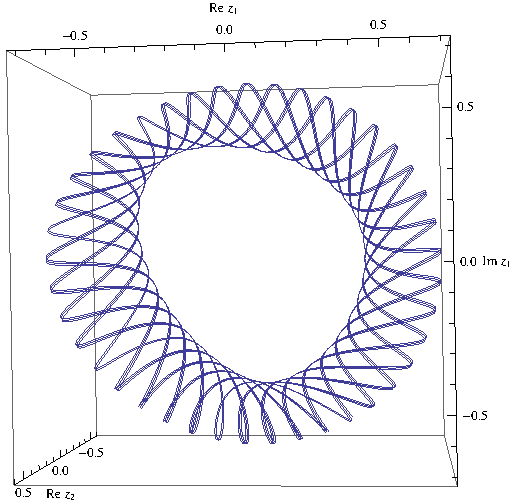
\includegraphics[width=0.35\textwidth]{dangelmayrProj}
\caption{Dangelmayr projected}
\label{fig:dangelmayr_proj}
\end{figure}

\item[2012-04-24 Predrag to Lei]

\begin{itemize}
%  \item can you svn add dangelmayrProj.pdf? (using underscores in LaTeX
%        files is awkward).
  \item stability eigenvalues, eigenvectors of the \eqv\ $\EQV{0}$ at
        origin, at your parameter values - if it is stable, everything
        just might fall into it and die.
  \item stability eigenvalues, eigenvectors of $\REQV{}{1}$
  \item stability eigenvalues, eigenvectors of $\REQV{}{2}$
  \item $\REQV{}{1}$: unstable eigenvalue becomes a complex
        eigenvalue pair in Cartesian coordinates?
  \item $\REQV{}{2}$: Does the unstable eigenvalue become a complex
        eigenvalue pair in Cartesian coordinates?
  \item their plots in the Cartesian coordinates
  \item $\dot{\theta}$ to see how slow/fast are they.
  \item plots of small perturbations of the above \eqv\ and \reqva\ in
        the Cartesian coordinates to see whether the dynamics looks
        chaotic
\end{itemize}

\item[2012-04-25 Lei to Predrag] In polar coordinates
\begin{description}
\item[$\REQV{}{1}$] $(r_1,r_2,\psi)=(0.712184,0.322201,-0.919559)$
\item[Eigenvalues] ${0.500667 \pm 1.87481i, 0.411071}$,
\item[Eigenvectors] $\{ \Re \jEigvec[1], \Im \jEigvec[1], \jEigvec[3]\}$ =\\
$(0.17281, 0.100144 , 0.939794)$,\\
$(-0.095779, 0.260235, 0)$, \\
$(-0.560937, -0.380607, 0.735179)$
\item[$\REQV{}{2}$] $(r_1,r_2,\psi)=(1.24041,0.357653,-0.238384)$
\item[Eigenvalues] ${3.20719, 0.259474 \pm 2.44789 i}$
\item[Eigenvectors]  $\{ \jEigvec[1], \Re \jEigvec[2], \Im \jEigvec[2]\}$ =\\
$(-0.0393065, -0.102858, 0.993919)$, \\
$(0.127876, 0.628119, -0.229194)$, \\
$(- 0.56813, 0, 0.462399)$
\end{description}


\item[2012-04-25 Predrag] \refFig{fig:dangelmayr_proj} is not chaotic -
it simply says that one of your \reqva\ (plot them both in
\reffig{fig:dangelmayr_proj}) is undergone a Hopf bifurcation into a
stable limit \rpo\ that you have plotted. Keep changing parameters so
this \rpo\ goes unstable and begets chaos.

\item[2012-04-25 Lei]
In cartesian coordinates, there seems to be no \eqv\ points.

\item[2012-04-24 Keith to Lei]  Isn't the origin an \eqv?  And the
periodic orbits shouldn't be a problem, since once we reduce they become
\eqv.

\item[2012-04-25 Lei]
All \eqva\ points in the reduced (set $\psi=2\theta_1-\theta_2$)
polar coordinates are actually \po s in original coordinates.

\item[2012-04-25 Predrag]  The flow is $\SOn{2}$-equivariant, so there
cannot be any \eqva\ and/or \po s that do not belong to a flow-invariant
subspace - this is {\color{red} the reason why we chose}
$\SOn{2}$-equivariant, not $\On{2}$-equivariant system to study. These
are {\color{red} not} \po s, these are \reqva. Please study the atlas
paper and ChaosBook chapter on continuous symmetries. A \reqv\ is a lazy
drifter, a \rpo\ is a bold dancer.

We need $\dot{\gSpace}$ for each of the two \reqva. Always list it when
you describe a \reqv.

$\REQV{}{2}$ seem to have insanely unstable real
eigenvalue, nothing probably comes close to it.

Is the complex eigenvalue pair of $\REQV{}{2}$ really mixing $r_1$ and $\psi$?
Fascinating - like bricks and cats, one has dimension of length, the other is
a dimensionless angle?

\item[2012-04-25 Evangelos] Not sure its a good idea to compute stability
of relative equilibria in polar coordinates, even though it is easier to locate
relative equilibria in polar coordinates. I think one should do what we did
in \refref{SCD07}.

\item[2012-04-25 Evangelos] Dangelmayr system with Predrag's modification
becomes very interesting. It's very easy to find chaotic behavior and in many
cases it seems that asymptotic dynamics are $3$-dimensional.
After spending some time playing with parameters, I've found some
for which it seems we have chaos (at least we can see some stretching
and folding) while a $2$-dimensional description might be possible
(a simple $2$-d branched manifold).
The parameters are
\[
 \mu_1 = -0.337,\, \mu_2 = 0.27,\, c_1 = 1,\, c_2 = -1,\, a_1 = -1.5,\,
 a_2 = -6.19,\, b_1 = 1.583,\,  b_2 = -0.115,\, e_2 = 1.211\,.
\]
I would suggest playing with \texttt{siminos/cgang/Evangelos/dangelmayr\_so2\_int.nb}
to locate \emph{nearby} parameters which you think will give more interesting
results or just explore the system with the parameters given here.

%%%%%%%%%%%%%%%%%%%%%%%%%%%%%%%%%%%%%%%%%%%%%%%%%%%%%%%%%%%%%%%%%%%%%%%%%%%%%%%%%%%%
 \begin{figure}
%% ES created with siminos/cgang/Evangelos/dangelmayr_so2_plot.nb
\centering
 (a) 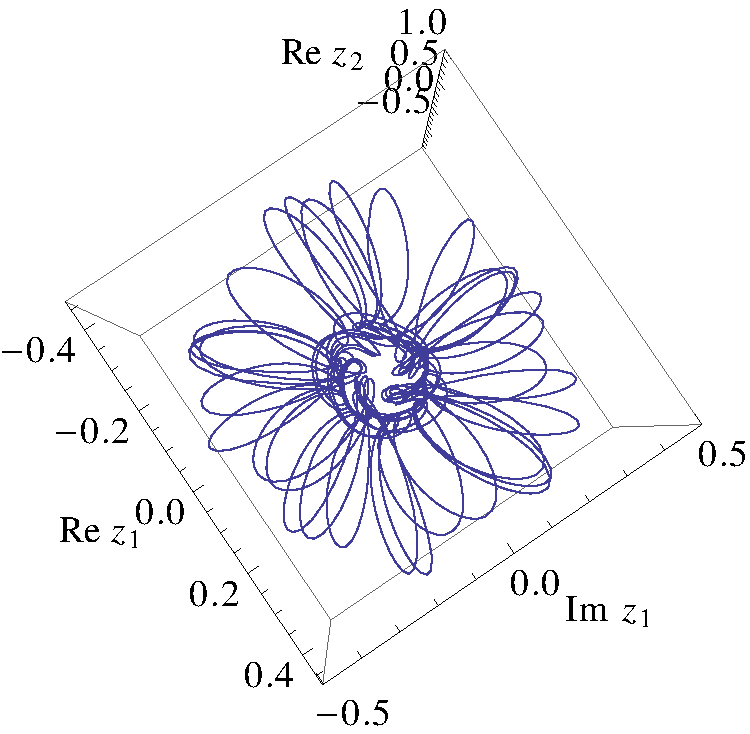
\includegraphics[width=0.35\textwidth]{dangelmayrZ}~
 (b) 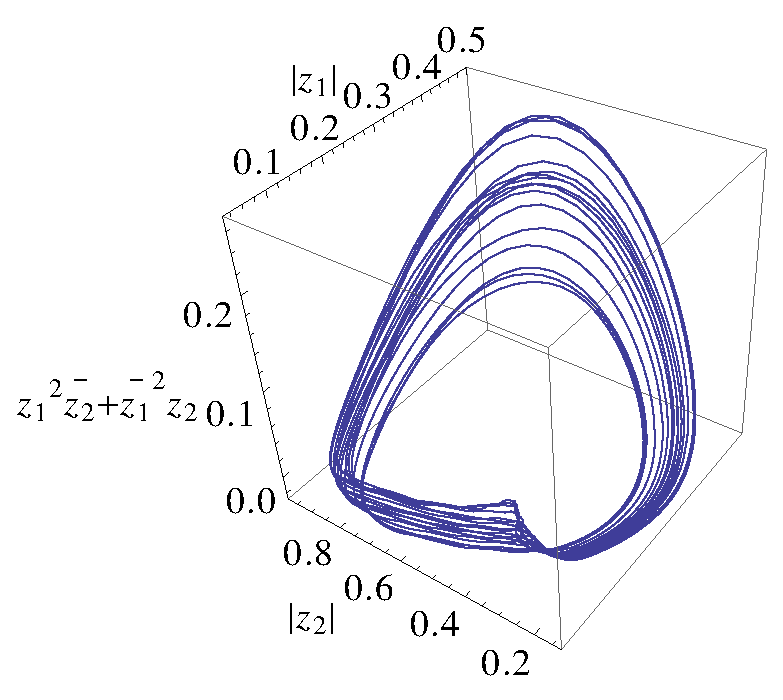
\includegraphics[width=0.35\textwidth]{dangelmayrAGH}~
\caption{Projections of Dangelmayr system \refeq{eq:DangSO2}
``attractor'' for $\mu_1 = -0.337,\, \mu_2 = 0.27,\, c_1 = 1,\, c_2 =
-1,\, a_1 = -1.5,\, a_2 = -6.19,\, b_1 = 1.583,\,  b_2 = -0.115,\, e_2 =
1.211$
(a) in original state space variables $\Re z_1,\,\Im z_1,\,\Re z_2$.
(b) in invariant coordinates used by
Armbruster \etal\rf{AGHO288} $|z_1|,\, |z_2|,\, z_1^2 \bar{z}_2 + \bar{z}_1^2 z_2$.
}
 \label{fig:dangelmayrChaos}
\end{figure}
%%%%%%%%%%%%%%%%%%%%%%%%%%%%%%%%%%%%%%%%%%%%%%%%%%%%%%%%%%%%%%%%%%%%%%%%%%%%%%%%%%%%%

\item[2012-04-05 Predrag to {\twoMode} gang] before we get into the habit of
calling it `Dangelmayr system': His had $\On{2}$ symmetry, we study a
related normal form with only  $\SOn{2}$, hence I've been using the
neutral but boring `{\twoMode}' appellation. As it is the custom name
something after a person who has not done it, I have no serious
objections to `Dangelmayr system'.

\item[2012-04-25 Evangelos to Predrag] It should most probably called
{\twoMode} system, see {\bf [2012-04-21 Evangelos]}. Until some
volunteer in the gang establishes the connection to {\twoMode}
system by computing the relation of their parameters to ours, I
tentatively call it Dangelmayr system, since this is how you introduced
it in \refeq{eq:AGpolar}.

\item[2012-04-25 Predrag to {\twoMode} gang] continuing on the discussion
above, of {\bf [2012-04-05 Lei to Predrag]}, a simple algebra question:
you say there are 20 complex solutions for \eqva\ + \reqva, with \reqva\
overcounted as you allow $\{\pm r_1, \pm r_2\}$. Can you count how many
distinct complex roots are there? That perhaps tells you what is the maximal
number of \template s this model could have. If we know the order of the
polynomial, you can track the roots in the complex plane, see for what
parameter values they go real. Evangelos might already know the answer,
because if you rewrite the {\twoMode} system in terms of Armbruster invariant
polynomials, there is no $\pm r_i$ problem.

\item[2012-04-05 Predrag to {\twoMode} gang] Really happy to see
\reffig{fig:dangelmayrChaos}! Seeing chaos is a start, but not enough.
\reffig{fig:dangelmayrChaos} seems to be a result of a Hopf \rpo\
bifurcated off a \reqv\ going chaotic (please, always plot all the
\reqva). That's going to be not more interesting than the \cLf. We need
chaos that visits qualitatively different templates in the pedagogically
simplest setting: a more complicated example, waiting to be sliced, are
the \eqva\ + \reqva\ of \refref{SCD07}. The only example where 2-chart
atlas of 2 sections (no continuous symmetry) was constructed is
\refref{lanCvit07} (click
\HREF{http://www.cns.gatech.edu/~predrag/papers/preprints.html\#ks}{here}).
You can see what templates should be by a glance at Fig.~1. The central
template's chart (Fig. 8) worked out beautifully. I never managed to get
across to Lan as to how to chart the second template neighborhood (Fig.
9, with a stunningly long \po), so we did not publish that return map (it
might be in Lan's thesis). We were still using Fourier modes as
coordinates then (stupid, stupid), and the \poincBord s and ridges were
yet undreamed of - that is the key contribution of the current C Gang
paper.

\item[Evangelos to Lei] In  [2012-04-05 Lei to Predrag] you say you get a
10th order polynomial equation for relative equilibria. Could you please
enter it here?

\item[2012-04-26 Lei to Keith] Yes. Zero should be a \eqv. I just
omit it by manipulating algebraic equations...

%\item[2012-04-26 Lei to Evangelos] I use the first two equations in the
%polar coordinates and eliminate $\psi$:
%\bea
% \frac{(\mu_1 r_1+a_1 r_1^3+b_1 r_1 r_2^2)^2}{c_1^2 r_1^2 r_2^2}
%+\frac{r_2^2 e^2}{(c_1 r_1^2+2 c_1 r_2^2)^2}  &=& 1
%    \continue
% \frac{(\mu_2 r_2+a_1 r_1^2 r_2+b_2 r_2^3)^2}{c_1^2 r_1^4}
%+\frac{r_2^2 e^2}{(c_2 r_1^2+2 c_1 r_2^2)^2}  &=& 1
%\label{2modeRequa1}
%\eea
%
%\item[2012-04-26 Predrag to Lei] I guess the program does not know how to simplify:
%\bea
% \frac{(\mu_1 +a_1 r_1^2+b_1 r_2^2)^2}{c_1^2 r_2^2}
%+\frac{r_2^2 e^2}{(c_1 r_1^2+2 c_1 r_2^2)^2}  &=& 1
%    \continue
% \frac{r_2^2 \, (\mu_2 +a_1 r_1^2 +b_2 r_2^2)^2}{c_1^2 r_1^4}
%+\frac{r_2^2 e^2}{(c_2 r_1^2+2 c_1 r_2^2)^2}  &=& 1
%\label{2modeRequa2}
%\eea
%\bea
% \frac{(\mu_1 +a_1 u+b_1 v)^2}{c_1^2 v}
%+\frac{v e^2}{(c_1 u+2 c_1 v)^2}  &=& 1
%    \continue
% \frac{v \, (\mu_2 +a_1 u +b_2 v)^2}{c_1^2 u^2}
%+\frac{u_2 e^2}{(c_2 u+2 c_1 v)^2}  &=& 1
%\label{2modeRequa3}
%\eea
%At this point I stop: please confirm there is no type in the
%second terms' denominators?


\item[2012-04-26 Daniel] Probably old hat at this point but I'm writing
the equations for the {\twoMode} system in case they ever come in handy.
Here's Siminos's \refeq{eq:DangSO2} in terms of 4 real variables,
such that $z_1 = x_1 + i x_2$ and $z_2 = y_1 + i y_2$. I did the algebra
using Matlab's symbolic math toolbox, so these should be correct.
\bea
\dot{x}_1 &=& a_1 x_1^3 + b_1 x_1 y_1^2 + c_1 x_1 y_1 + a_1 x_1 x_2^2 + b_1 x_1 y_2^2 + \mu_1 x_1 + c_1 x_2 y_2
\continue
\dot{y}_1 &=& a_1 x_1^2 x_2 + c_1 x_1 y_2 + b_1 y_1^2 x_2 - c_1 y_1 x_2 + a_1 x_2^3 + b_1 x_2 y_2^2 + \mu_1 x_2
\continue
\dot{x}_2 &=& a_2 x_1^2 y_1 + c_2 x_1^2 + b_2 y_1^3 + a_2 y_1 x_2^2 + b_2 y_1 y_2^2 + \mu_2 y_1 - c_2 x_2^2 + e_2 y_2
\continue
\dot{y}_2 &=& a_2 x_1^2 y_2 + 2 c_2 x_1 x_2 + b_2 y_1^2 y_2 - e_2 y_1 + a_2 x_2^2 y_2 + b_2 y_2^3 + \mu_2 y_2
\label{2mode4D}
\eea

\item[2012-04-26 Daniel to Evangelos] Just tried to figure out how the parameters
in our {\twoMode} system \refeq{eq:DangSO2} are related to the paramters
in {\twoMode} $SO(2)$-symmetric equations and found that they do not
map directly (or perhaps you made a mistake copying your results into the blog).
P\textit{\&}K's equation for $\dot{z_2}$ has a linear term in $z_2$ and no linear
term in $z_1$. I don't have access to the original Dangelmayr paper, so I can't
check that one, but Armbruster et al.\rf{AGHks89} also have this term.
Our $\dot{z_2}$ has a linear term in $z_1$ but no linear term in $z_2$.
I guess if you are seeing chaos in our system, it might be fine, but for a
larger audience we might want the P\textit{\&}K or AG\textit{\&}H systems.
Let me know if you've made a mistake and I'll recalculate the various equations
in 4D and polar coordinates.

\item[2012-04-26 Evangelos to Daniel] That was a typo in \refeq{eq:DangSO2}, sorry,
fixed now. There is no error in my Mathematica files, which use the correct
Dangelmayr equations (which are also the starting point for P\textit{\&}K)
and the parameters used in the figures are also correct. But it would be a
good idea if someone else checked to see what the attractors look like.

\item[2012-04-26 Evangelos] Added Dangelmayr paper\rf{Dang86} in CNS zotero library.

\item[2012-04-26 Predrag to Evangelos] Zotero says ``The attached file
could not be located ...''

\item[2012-04-27 Evangelos] Maybe we run out of space. I'll check
tommorow, meanwhile I'll email it to you.

\item[2012-04-26 Predrag] Thanks! I put it
\HREF{http://ChaosBook.org/library/Dang86.pdf}{here}. This version is
better than Evangelos', as I have made it text-searchable and a bit
smaller than the journal download.

Dangelmayr paper\rf{Dang86} is a serious, detailed paper on normal forms
for bifurcations, and quite interesting. I like his concise statement of
invariance and equivariance. Invariant polynomials in 2 complex
dimensions are so seductive, wish they were good also for 10's or 100's
of dimensions...

Which student is going to (gasp!) read it, and (gasp! gasp!) blog about
it?

Dangelmayr considers a  system constructed from two arbitrary Fourier modes,
a representation
of the symmetry group $\On{2}$ which is defined by the operations of
rotation and reflection,
\begin{subequations}\label{Dang86(1.1)}
\beq
(z_1,z_2) \rightarrow   (e^{im {\gSpace}}z_1,e^{in {\gSpace}} z_2)
\ee{Dang86(1.1)a}
\beq
(z_1,z_2) \rightarrow   (\overline{z}_1,\overline{z}_2)
\,,
\ee{Dang86(1.1)b}
\end{subequations}
respectively, acting on complex vectors $(z_1,z_2) \in \complex^2 \simeq
\reals^4 $. Here, $m, n$ are positive integers where $(m, n)$ satisfies
either $2 \leq m < n$ with  $(m, n)$ relatively prime or $m = 1 <n$, and
the bar denotes complex conjugation. He cites an unpublished preprint by
Buzano and Russo for establishing that there are three basic functions
that are invariant under \refeq{Dang86(1.1)},
\beq
u = {z}_1\,\overline{z}_1
    \,,\quad
v = {z}_2\,\overline{z}_2
    \,,\quad
w = z_1^n \overline{z}_2^m + \overline{z}_1^n {z}_2^m
\,.
\label{Dang86(1.2)}
\eeq
and that the basic equivariants are
\beq
  \{{z}_1\,,\overline{z}_1^{n-1} {z}_2^m\}
            \,,\qquad
  \{{z}_2 \,, z_1^n \overline{z}_2^{m-1}\}
\,.
\label{Dang86(1.3)}
\eeq
Buzano and Russo  published papers are tedious, we do not need to
cite them - all about buckling rods, citing only Dangelmayr is fair
enough.
Any invariant function can be represented as $f(u,v, w)$ for some $f :
\reals^3 \to \reals$. A general smooth mapping $\complex^2  \to
\complex^2$ can be constructed in terms of the basic equivariants by
multiplying each of the vectors in \refeq{Dang86(1.3)} by a general
invariant function and then adding the resulting terms. In this way we
obtain the following form for a general smooth vector field which is
equivariant under \refeq{Dang86(1.1)}:
\bea
  \dot{z}_1 &=& p_1\,z_1+q_1\,\overline{z}_1^{n-1} {z}_2^m
            \continue
  \dot{z}_2 &=&  p_2\,z_1+q_2\,z_1^n \overline{z}_2^{m-1}
\,,
\label{Dang86(1.4)}
\eea
where $p_j,q_j$ are smooth invariant functions, that is, \emph{real
functions} of $u, v, w$ and any external parameters.
The cases in which $m = 1$ and $m > 1$ give rise to rather distinct
behaviour. Also, the case where $m = 1$ must be further distinguished
according to whether $n = 2$ or $n > 2$. Dangelmayr discusses $(m,n ) = (
1 ,2)$ and $m > 2$ cases.

We consider here only the simplest normal form of the $(m,n ) = ( 1 ,2)$ case,
and go from  $\On{2}$ to  $\SOn{2}$ by taking some parameters complex,
and thus breaking the reflection invariance, $\dot{\overline{z}}_j \neq
\dot{\overline{f}}_j \,.$ As Dangelmayr consider only the real case,
calling our system a special case of {\twoMode} is fair enough.

\item[2012-04-21 Evangelos]
The Dangelmayr system\rf{Dang86} written in complex coordinates $z_1,z_2$
is given in \refeq{eq:DangSO2} I have replaced symmetry breaking term $e$
here and in \refeq{eq:AGpolar} with $e_2$ since in this constant is
naturally paired with $\mu_2$. See also Armbruster, Guckenheimer and
Holmes\rf{AGHO288} flow with $\On{2}$ symmetry, here \refeq{eq:AGH}. In
\texttt{siminos/cgang/Evangelos/dangelmayr\_so2\_int.nb} I integrate
\refeq{eq:DangSO2} rather than the polar form \refeq{eq:AGpolar}, as the
former has no dangerous denominators.

\item[2012-04-21 Evangelos] For future reference I note that the
connection of the constants in \refeq{eq:DangSO2} with $e_2=0$ to the
constants in equation (2.3) of \refref{Dang86} with
$n=2$, $m=1$ is $\mu_1=\nu\epsilon\alpha$,
$a_1=-\nu\epsilon$, $b_1=-\nu\epsilon\rho$, $c_1=-\nu\mu$, $\mu_2=\epsilon\beta$,
$a_2=-\epsilon\kappa$, $b_2=-\epsilon\epsilon'$, $c_2=\mu\mu'$.

\item[2012-04-27 Predrag]
% because I stood on shoulders of Dangelmayr:
% There is this really cool book,\rf{DasBuch} so I'll just follow it.
$\SOn{2}$ is a {subgroup} of $\On{2}$, without the reflection group
element \refeq{Dang86(1.1)b}. As a subgroup, it has to satisfy invariance
constraints in addition to those of $\On{2}$, with one more invariant
polynomial in its basis, called $q$ in what follows. The
stand-alone write up is now in \refsect{s:twoMode}.


\item[2012-04-27 Predrag] This could be more elegant - I made only
$(\mu_2-\ii\, e_2)$ imaginary, and I am not sure why I am breaking the
reflection symmetry of $m=2$ mode (that also breaks it in the $m=2$
flow-invariant subspace), but that's what we have done so far. Finding
\eqva\ using these equations should be easy - they are like the polar
equations but more elegant, extracting $\dot{\psi}$ is silly - $w$, $q$
tell you you want equations for $(\cos \psi, \sin \psi)$ instead.

\item[2012-04-28 Evangelos] Indeed, using \refeq{PKinvEqs1} should be the
cleanest way to compute relative equilibria, as equations are given in
a clear polynomial form.
To find relative equilibria in $u,v,w,q$ basis
one would have to solve $\dot{u}=\dot{v}=\dot{w}=\dot{q}=0$ in \refeq{PKinvEqs1}
together with the syzygy \refeq{eq:syzPK} [$\left(\frac{w}{\DBedit{2}}\right)^2+\left(\frac{q}{\DBedit{2}}\right)^2 - u^2v =0$], right?
In other words, \refeq{eq:syzPK} is a constraint in allowable solutions which
dynamics knows about, but when solving algebraic equations for (relative)
equilibria, don't we have to impose it?

\item[2012-04-25 Evangelos] Yet another snapshot of {\twoMode}
system with Predrag's modification, for different parameters. This looks
like an attractor made of two pieces, so it might be complicated enough
to demonstrate slicing. However I have yet no insight on whether there
are really two distinct topological mechanisms hidden here and what
controls them. Once relative equilibria are located, we should add them
here. The parameters are
\[
 \mu_1 = -0.337,\, \mu_2 = 0.27,\, c_1 = 1,\, c_2 = 1,\,
 a_1 = -0.4,\, a_2 = -6,\, b_1 = 1.6,\,  b_2 = -0.1,\, e_2 = 1.217
 \,.
\]

%%%%%%%%%%%%%%%%%%%%%%%%%%%%%%%%%%%%%%%%%%%%%%%%%%%%%%%%%%%%%%%%%%%%
 \begin{figure}[h]
%% ES created with siminos/cgang/Evangelos/dangelmayr_so2_plot.nb
\centering
 (a) 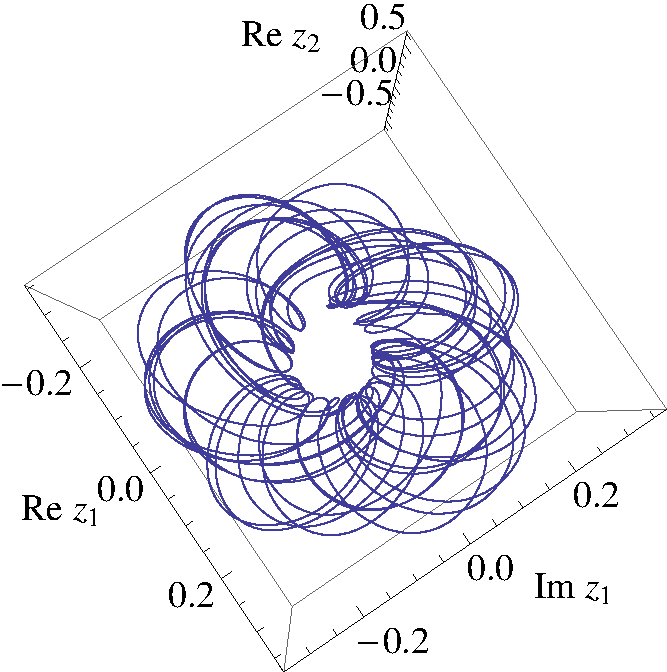
\includegraphics[width=0.35\textwidth]{dangelmayrZ2}~
 (b) 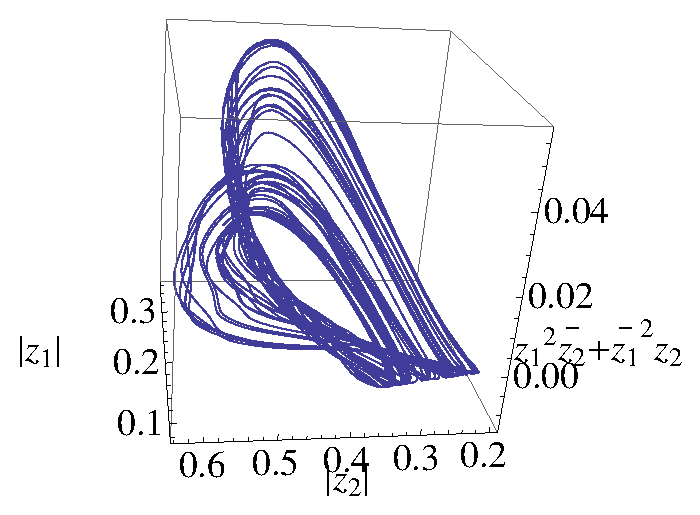
\includegraphics[width=0.35\textwidth]{dangelmayrAGH2}~
\caption{Projections of Dangelmayr system \refeq{eq:DangSO2}
``attractor'' for $\mu_1 = -0.337,\, \mu_2 = 0.27,\, c_1 = 1,\, c_2 = 1,\,
a_1 = -0.4,\, a_2 = -6,\, b_1 = 1.6,\,  b_2 = -0.1,\, e_2 = 1.217\,.$
(a) in original state space variables $\Re z_1,\,\Im z_1,\,\Re z_2$.
(b) in invariant coordinates used by
Armbruster \etal\rf{AGHO288}
$|z_1|,\, |z_2|,\, z_1^2 \bar{z}_2 + \bar{z}_1^2 z_2$.
}
 \label{fig:dangelmayrChaos2}
\end{figure}
%%%%%%%%%%%%%%%%%%%%%%%%%%%%%%%%%%%%%%%%%%%%%%%%%%%%%%%%%%%%%%%%%

\item[2012-04-27 Predrag] \refFig{fig:dangelmayrChaos2}\,(b) is one of 4
projections from the 4\dmn\ invariant polynomials $\{u,v,w,q\}$ dynamics
on any three of them. I would prefer that all such projections are linear
in coordinates (otherwise small $z_i$ really get scrunched), so please
plot $\{|u|^{1/2},|v|^{1/2},w/u |v|^{1/2} ,q/u |v|^{1/2} \}
= \{r_1,r_2, \cos\psi, \sin\psi \}$, or similar...

\item[2012-04-27 Predrag to Chaos Gang] That sinking feeling...

OK, I learned my lesson:
\HREF{http://www.flickr.com/photos/birdtracks/6971784058/in/set-72157607005727427/}
{you} do not write. The game plan is to abuse a defenseless assistant
professor who must publish. She will write your articles for you in grad
school, and then you'll be on the street again.

But, do you read? In your project you are referencing several impressive,
well written {\twoMode} articles, where some of the problems you are
encountering are discussed and solved. Ethos of the profession is that if
one references a publication, one has read it, and the key ones one has
studied in depth. OK, not all of us have read \emph{Principia} (I did it
for the high school senior project, that was before we had smart phones,
and even then I did not understand anything), but we do not cite it
either. And it gets fuzzy in collaboration, as not all contributors
contribute to everything. But then at least one of the coauthors can
explain what a given cited paper says.

\item[2012-04-26 Daniel] Uploaded code to
\texttt{/siminos/cgang/Daniel/Matlab/}. Just type \texttt{EOMComplexTo4D}
at the Matlab prompt and it will calculate the system in 4D Cartesian, 4D
polar, and 3D polar coordinates. The $\dot{z_j}$ equations can be
modified within the code if need be.

For future reference, our {\twoMode} system \refeq{eq:AGpolar} is a
special case ($\omega_1 = 0$) of the system of Porter and
Knobloch\rf{PoKno05}. Our parameters are related to their parameters by
(P\textit{\&}K $\leftrightarrow$ ChaosGang {\twoMode}):

\(
  \mu_1 \leftrightarrow \mu_1,\, \epsilon \omega_1 \leftrightarrow 0,\,
  \tilde{\alpha} \leftrightarrow c_1,\, \tilde{d}_{11} \leftrightarrow a_1,\,
  \tilde{d}_{12} \leftrightarrow b_1,\, \mu_2 \leftrightarrow \mu_2,\,
  \\
  \epsilon \omega_2 \leftrightarrow -e_2,\, \tilde{\beta} \leftrightarrow c_2,\,
  \tilde{d}_{21} \leftrightarrow a_2,$ and  $\tilde{d}_{22} \leftrightarrow b_2
\,.
\)

\item[2012-04-27 Evangelos] Great, it wasn't so terrible after all. So
now we can call this system Porter-Knobloch flow.

\item[2012-04-27 Evangelos to Daniel and the gang]
I think since Porter and Knobloch  use complex parameters,
our model is a special case of theirs with
$\omega_1=\alpha_i =\beta_i=c_{11}=c_{12}=c_{21}=c_{22} = 0$
and correspondence of parameters:

 $\mu_1 \leftrightarrow \mu_1,\, \alpha_r \leftrightarrow c_1,\, d_{11} \leftrightarrow a_1,\, d_{12} \leftrightarrow b_1,\, \mu_2 \leftrightarrow \mu_2,\, \epsilon \omega_2 \leftrightarrow -e_2,\, \beta_r \leftrightarrow c_2,\, d_{21} \leftrightarrow a_2,$ and  $d_{22} \leftrightarrow b_2$.

\item[2012-04-27 Evangelos] If we let $\omega_1\neq0$ we might generate
some interesting dynamics (by adding an extra frequency we might gain an
extra \reqv).

\item[2012-04-26 Daniel to Chaos Gang] Sorry to keep raining on the
party, but I believe \refeq{eq:AGpolarREQV} have another typo in
them. If you take \refeq{eq:AGpolar} and set them to zero, you end
up with a $b_1 r_2^2$ term in the equation for $\dot{r}_1$ rather than
$b_1 r_1 r_2$ term. This is confirmed by my \texttt{EOMComplexTo4D.m}
code using \refeq{eq:DangSO2} as a starting point. If you are
working on the {\twoMode} \reqva, you probably want to stop and
double check this before moving on but I'm pretty sure I'm right. {\bf To
Lei:} Did you derive \refeq{2modeRequa4} from \refeq{eq:AGpolar}
or from \refeq{eq:AGpolarREQV}? If it was the latter, you probably
want to double check it.

\item[2012-04-27 Evangelos] Daniel is correct, I have the same term in my notes.

\item[2012-04-27 Keith]  I have developed a program that finds zeros of
the equations we have (it disregards imaginary solutions).  About half of
them actually come up as \reqva, and these are nice and
the trajectories that I start on these stay one these; the other
solutions are not doing this at all.  I am checking the conditions we
have about the flow being in the same direction as the tangent and only
some of them meet the requirements.  I am wondering if using the squared
versions of the equations is introducing more solutions than there truly
are.  The other thought I am having is if this squaring could be
introducing problems with the phases being offset by $\pi$ or others.


\item[2012-04-27 Keith]  I spent some time really thinking about this,
and I just tested it.  You can't just use the squared equations,
\refeq{2modefixdenom}, that we have, you need to also go back and verify
it solves the original equation \refeq{eq:AGpolarREQV}, otherwise you
come up with strange solutions that almost act as \reqva\
but they are not.  I have tried to see if adding phase factors will
adjust this, but it appears not.  Does anyone have an insight as to why
this is?  It is probably something simple.

 \begin{figure}[h]
\centering
  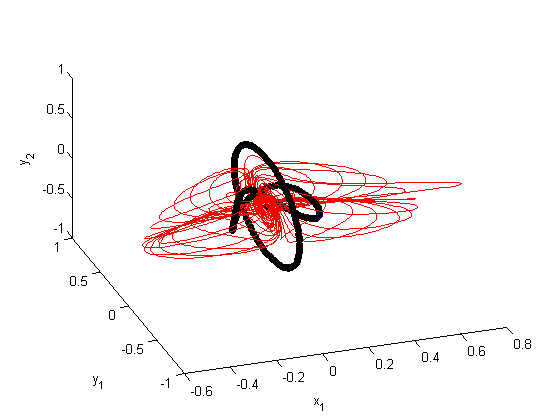
\includegraphics[width=0.45\textwidth]{kc2mode.png}
\caption{
Possibly what we are looking for in the {\twoMode} system.  Red labels the
trajectory, black labels the \reqv.}
 \label{fig:2modeproblem}
\end{figure}

\item[2012-04-27 Keith] So I toyed around with a bunch of things and kept
twisting parameters, and eventually got this \reffig{fig:2modeproblem}.
I can give you the eigenvalues/vectors and \reqv.  I
also have the parameters and I twisted them, not a computer.  I want to
plot it in \reducedsp, but I need to go eat first.  I just want to get
this out there before I do that.  I think this has the elements we are
looking for.  The trajectories are spiralling around one the of the
\reqva, and if you look close enough they are spiralling
around the \eqv\ at the origin.  I plotted this in 4-d space, and
in hind sight should have done the polar coordinates, but for now I think
this image captures what I have.


\item[2012-04-27 Keith] There is one problem, and its in a
couple of the papers, but if you start on $r_1 = 0$ you stay on it and
tend to approach the \reqv\ in that space, but this is OK,
I think.

\item[2012-04-27 Predrag] It's no problem, mon $\cdots$ just a situation.
It's a flow invariant subspace.


\item[2012-04-27 Bryce] I'm in the process symmetry reducing the flow
myself but in the meantime I wanted to verify a couple of things. Under
what rotation is the Dangelmeyr system invariant? That is to say which
entries of generator (assuming one is working in $\{x1, y1, x2, y2\}$ coords.)
are zero/one? Keith: which parameters did you use to produce
\reffig{fig:2modeproblem}?


\item[2012-04-27 Keith to Bryce] The parameters were bad.  They don't
have the trajectory visiting both equilibrium, it just looks that way.
If you still want them, Ill give them though.  Generator:

    \beq
\Lg  \, =
\left( \begin{array}{cccc}
         0 & 1 & 0 & 0 \\
        -1 & 0 & 0 & 0 \\
         0 & 0 & 0 & 2\\
         0 & 0 & -2 & 0
      \end{array} \right)
\,.
\ee{2modeGnrtr}
The minus sign may be switched, its the same as the \cLe.  But this should
be enough to get you started.

\item[2012-04-27 Predrag] The infinitesimal transformations
generator \refeq{2modeGnrtr} is correct.

\item[2012-04-27 Predrag to Daniel] As you did check the invariance by showing that
the Jacobian derivative,
\beq
  \groupTan_a(\vel)  - \Mvar(\ssp) \, \groupTan_a(\ssp) =0
  \,,
\ee{inftmInv}
vanishes, maybe you make it into problems set - solution like you did for
my original proto-{\twoMode}, it would be nice to have that explicitly in the
{\twoMode} project?

\item[2012-04-26 Predrag] On factoring polynomials (this is somewhere in
the blog of a few weeks ago, but perhaps now falling on more receptive
ears): {\twoMode} system has 2 invariant subspaces, $r_1=r_2=0$ and
$r_1=0$, $r_2\neq 0$, so you already know two roots of your polynomial;
the $u=v=0$; and $u=0$, $\mu_2  +b_2 v =0$. Still do not know what the
order of this polynomial really is, but whatever polynomial you get, you
should \emph{divide it} by the roots you already know, that brings the
order of the polynomial down.

\item[2012-04-27 Daniel] I know that the Chaos Gang is zipping ahead into
uncharted territory, but here are some previously undocumented results
for meager fixed points and the easy \reqva.
	\begin{itemize}
		\item By using Matlab to symbolically solve  \refeq{2mode4D},
             I found that the only fixed point is the origin, independent
             of parameter choices.
{\bf [2012-03-31 Predrag]} Most solutions are `mixed modes'. However,
{\bf [2012-04-06 Predrag]}
there is an \eqv\ for $r_1=r_2=0$. There is a invariant subspace $r_1=0$,
$r_2 > 0$ which you can solve analytically - it my cause us some trouble.
If what you end up solving is a polynomial in $r_1$, you want to divide
it with all these known roots, see whether anything of interest is still
left. {\bf [2012-04-25 Predrag]} Obviously there is one \eqv, very
important one, for all $z_i=0$. Eigenvectors could be complex,
due to the $\SOn{2}$ equivariance of perturbations off the origin.
One eigenvector pair must belong to the $m=2$ invariant subspace, the other
should be pure $m=1$, as at the origin linear theory
of irreducible representations applies (reread ChaosBook.org Sect.~10.3
\emph{Stability}).
             The eigenvalues are $\lambda_1 = \mu_1$ with multiplicity 2 and
             $\lambda_2 = \mu_2 \pm i e_2$. The eigenvectors for
             $\lambda_1$ are $(1,0,0,0)$ and $(0,1,0,0)$ in the
             $(x_1,x_2,y_1,y_2)$ basis. The complex eigenvectors for
             $\lambda_2$ are $(0,0,\mp i, 1)$. {\bf [2012-04-25 Predrag]}
             One always replace complex eigenvector pair by  $\{\Re
             \jEigvec[j], \Im \jEigvec[j]\}$: that defines the real plane
             in which spiral-out takes place.
             The eigenvectors for
             $\lambda_2$ thus are $(0,0,1,0)$ and $(0,0,0,1)$
             % Notice the exchange of $\pm$ for $\mp$ in going from
             % eigenvalues to eigenvectors.
             I have uploaded the code that generated these as
             \texttt{/siminos/cgang/Daniel/Matlab/TwoModeOriginStability.m}
		\item {\bf [2012-04-27 Predrag]} As we want hyperbolicity, pick $\mu_j$
             of opposite signs. In order to avoid the \cLe\ near visits to
             the invariant subspace (there it was the $z$ axis, here it is the
             $m=2$ subspace) pick contraction within the subspace, $\mu_2 < 0$, but
             make it overall repelling by making sure that $\mu_1 > -\mu_2 > 0$.
             No parameters that you have reported chaos for so far satisfy that.
		\item I also started going after \reqva. The first (and obvious)
             is in the $r_1 = 0,\, r_2 > 0$ invariant subspace. Starting from
             \refeq{eq:AGpolar}, I got that there are  \reqva\ at $r_1 =
             0, r_2 = \pm \sqrt{-\mu_2 / b_2}$, and $\psi =
             \sin^{-1}\left(\pm \frac{e_2} {2 c_1}
             \sqrt{\frac{-b_2}{\mu_2}}\right)$. Given the additional
             constraints that 							$r_2$ must be
             real and positive, I conclude that the \reqva\ reduce to a
             single one at
\(
\left(r_1,r_2,\psi\right) =\left(0,\sqrt{-\mu_2 / b_2},
             sin^{-1}\left(\frac{e_2}{2 c_1}
             \sqrt{\frac{-b_2}{\mu_2}}\right)\right)
\,,
\)
            which is only physical if $\mu_2 / b_2 < 0$ and
            $\left|\frac{e_2}{2 c_1} \sqrt{\frac{-b_2}{\mu_2}}\right|
            \leq 1$.
            \\
{\bf [2012-04-27 Predrag]} please compute its stability. As it is within
the repelling $m=2$ invariant subspace, it's existence and stability
probably does not matter much, but if you can make it unstable, do so.
	\end{itemize}

\item[2012-04-25, 2012-04-27 Predrag] Thanks! moved the earlier entries
that nobody read into your text.

\item[2012-04-25 Bryce] Nothing fancy here but I've written code to
symmetry reduce \refeq{2mode4D}. I am currently choosing a random slice
(no thinking yet!) just to see if it worked and the results were quite
surprising \reffig{fig:pkfig1}.

\begin{figure}[H]
\centering
 (a) 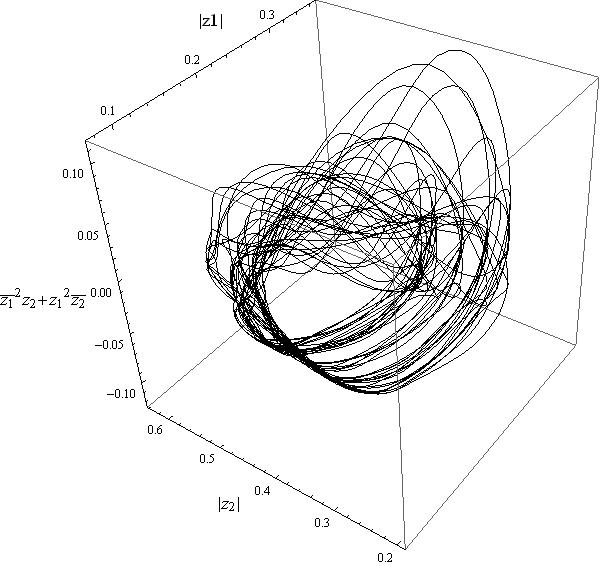
\includegraphics[width=0.35\textwidth]{pkTraj1}
 (b) 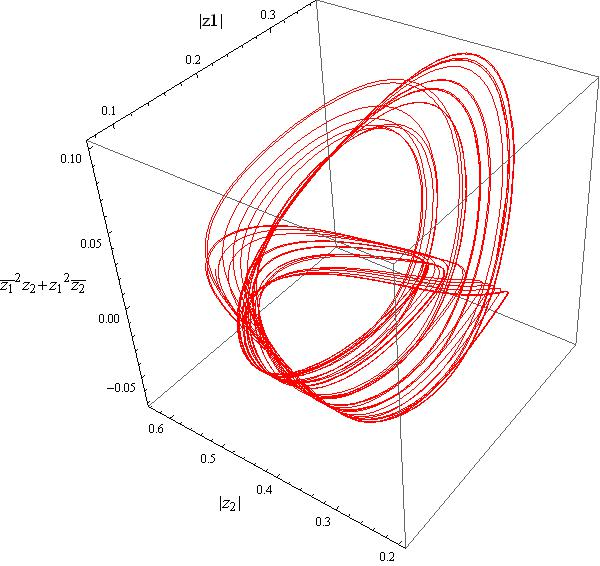
\includegraphics[width=0.35\textwidth]{pkTraj1Reduced}

\caption{Projection of Dangelmayr system \refeq{2mode4D}
``attractor'' for $\mu_1 = -0.337,\, \mu_2 = 0.27,\, c_1 = 1,\, c_2 =
1,\, a_1 = -1.4,\, a_2 = -6,\, b_1 = 1.6,\,  b_2 = -0.1,\, e_2 = 1.217$.
(a) Projection onto original state space:
$(|z_1|,|z_2|,z_1^2\overline{z_2}+\overline{z_1}^2 z_2)$. (b) Symmetry
reduced trajectory using the following template for the slice $(0.220299,
0.784274, -1.03596, 2.46552)$.
}
\label{fig:pkfig1}
\end{figure}

\item[2012-04-25 Bryce] In the spirit of ``experimenting'' I flipped the
sign of b2 from -0.1 to .01 and got the following plots. Not sure what to
make of them though... My brain needs some fuel and my eyes are starting
to strain so I'm throwing the towel in for now in favor of some food.

\begin{figure}[H]
\centering
 (a) 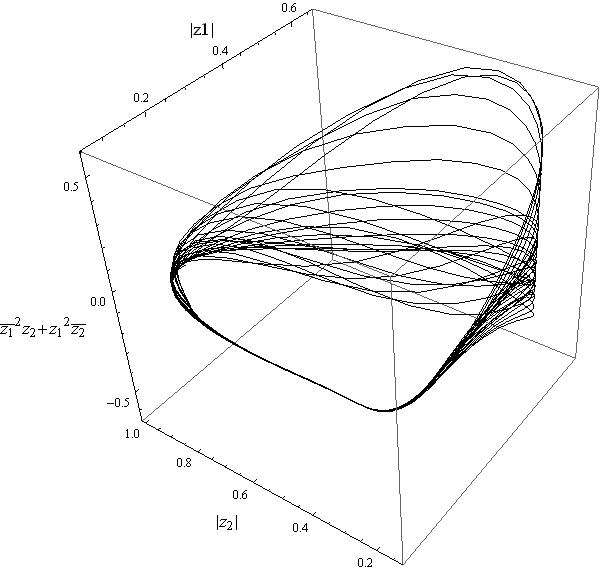
\includegraphics[width=0.35\textwidth]{pkTraj2}
 (b) 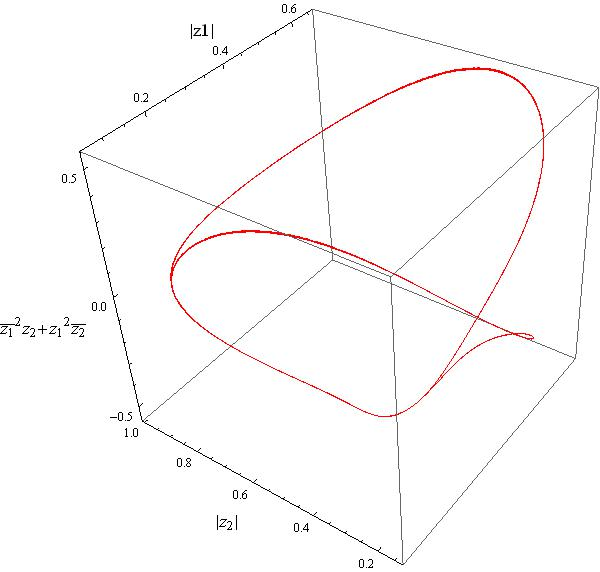
\includegraphics[width=0.35\textwidth]{pkTraj2Reduced}
\caption{Projection of Dangelmayr system \refeq{2mode4D}
``attractor'' for $\mu_1 = -0.337,\, \mu_2 = 0.27,\, c_1 = 1,\, c_2 =
1,\, a_1 = -1.4,\, a_2 = -6,\, b_1 = 1.6,\,  b_2 = 0.1,\, e_2 = 1.217$.
(a) Projection onto original state space:
$(|z_1|,|z_2|,z_1^2\overline{z_2}+\overline{z_1}^2 z_2)$. (b) Symmetry
reduced trajectory using the following template for the slice $(0.220299,
0.784274, -1.03596, 2.46552)$.
}
\label{fig:pkfig1}
\end{figure}

\item[2012-04-27 Predrag] Experimenting is great, but please read what I
have written, and either show me that I am wrong, or experiment
accordingly. Here are clips of above unread text:

(clip 1) As we want hyperbolicity, pick $\mu_j$ of opposite signs. In
order to avoid the \cLe\ near visits to the invariant subspace (there it
was the $z$ axis, here it is the $m=2$ subspace) pick contraction within
the subspace, $\mu_2 < 0$, but make it overall repelling by making sure
that $\mu_1 > -\mu_2 > 0$. No parameters that you have reported chaos for
so far satisfy that.

(clip 2) \refFig{fig:pkfig1}\,(b) is one of 4
projections from the 4\dmn\ invariant polynomials $\{u,v,w,q\}$ dynamics
on any three of them. I would prefer that all such projections are linear
in coordinates (otherwise small $z_i$ really get scrunched), so please
plot $\{|u|^{1/2},|v|^{1/2},w/u |v|^{1/2} ,q/u |v|^{1/2} \}
= \{r_1,r_2, \cos\psi, \sin\psi \}$, or similar...

\item[2012-04-27 Keith to Predrag] I know what your suggestions are for
$\mu_1$ and $\mu_2$, but I found the origin never to have much an effect
on any of the dynamics, so I went and tried some other stuff.  What I
found when I symmetry reduced was what appears to be two R\"ossler like
trajectories floating around two equilibrium and a single trajectory
visiting both: \reffig{fig:2moderedmultieq}.  I post processed this
trajectory rather than running the dynamics in the slice, and the slice
was: $[1, 0, 0, 0]$ which is rather unoriginal, but it provided the
easiest condition for rotating the frame at the time, because once I
found these parameters, I thought there might be some interesting events
to these.  The problem, of course with this slice is that the invariant
space $r_1 = 0$ remains a circle.
    The parameters are given as:
    $\mu_1 = 2.0 ,\, \mu_2 = 1.0,\, a_1 = -7.5,\, a_2 = -2,\,
      b_1 = -4,\,  b_2 = -2.25,\, c_1 = 10,\, c_2 = -35,\, e_2 = 2 \,.$

\item[2012-04-28 Predrag] Wow, this is beautiful. Victoria Secret's Pink
line. The three dots are the \eqv\ and two rather similar \reqva, both
spiral-out unstable? Is the $m=2$ subspace ($r_1 = 0,\, r_2 > 0$) \reqv\
where Daniel says it is? Stable, unstable? Whatever `slice' means (there
are rumors of a good paper defining it, but's not on arXiv yet), it is
not $[1, 0, 0, 0]$. No habla esta idioma. You mean template $\slicep =
[1, 0, 0, 0]$ or group tangent $\sliceTan{} = [1, 0, 0, 0]$? Presumably
$\sliceTan{} = [1, 0, 0, 0]$. Not obvious to me that \reqv\ in $m=2$
remain a circle, but there surely is one (attractive?) that seems to give
shape to the hot pants. You seem to have set $x_2=0$ (that is $m=2$
coordinate?)

Time to go to bed...

\item[2012-04-27 Keith]  I am still writing my own project up, I have
just been posting in here because everyone was working on the 2-mode, is
that alright?  I haven't been posting there because I focused on this for
a while, and haven't updated that one.  I do not know how much I need to
input in this one therefore, or if me going off and studying the return
map stuff is alright.

\item[2012-04-28 Predrag to Keith] Of course, the return
map stuff is important.

\item[2012-04-28 Lei to Predrag] Can I get access to Dangelmayr's paper?
It seems I don't know the password.

\item[2012-04-28 Predrag] cnsuser cnsweb

\item[2012-04-27 Predrag] Regarding \refeq{eq:DangSO2} in terms of 4 real
variables \refeq{2mode4D}- unfortunately for \cLe\ one writes $z_1 = x_1
+ i x_2$ and $z_2 = y_1 + i y_2$ (so rotations are in `x' and `y' planes
- this mixes them up). Might be confusing in the time to come.

\item[2012-04-28 Daniel] Well, it's sort of trivially easy fix. I just
thought I'd keep 1's together and 2's together since that's the way they
appear in eqs. \refeq{eq:AGpolar} and \refeq{eq:DangSO2}. Want me to
change them to $z_1 = x_1 + \ii x_2$ and $z_2 = y_1 + \ii y_2$? I would
take me 5 minutes. [2012-04-29 Daniel] Changed all 4D Cartesian representations
of $z_1$ and $z_2$ in blog and \emph{my} Matlab codes to be consistent with the substituion used in DasBuch for
the \cLe\ system as outlined by Predrag in the previous post.

\item[2012-04-28 Predrag] Low priority, but if only 5 minutes, do it sometime.

\item[2012-04-28 Predrag]
A stand-alone write up of invariant polynomials formulation of {\twoMode}
is now in \refsect{s:twoMode}. Edit and improve it there, in the project
proper.

\item[04-28-2012 Daniel]
%%%%%%%%%%%%%%%%%%%%%%%%%%%%%%%%%%%%%%%%%%%%%%%%%%%%%%%%%%%%%%%%%%%%%%%%%%%%%%%%%%%%%%%%%
\DBedit{Starting from the following definitions:}
\bea
u &=& {z}_1 \overline{z}_1
    \,,\quad
v = {z}_2 \overline{z}_2
    \continue
w &=& (z_1^2 \overline{z}_2 + \overline{z}_1^2 {z}_2)\DBedit{/2} %Otherwise equality doesn't hold
   = \Re(z_1^2 \overline{z}_2) = u |v|^{1/2} \cos \psi
    \continue
q &=& (z_1^2 \overline{z}_2 - \overline{z}_1^2 {z}_2)/2i
   = \Im(z_1^2 \overline{z}_2) = u |v|^{1/2} \sin \psi
\,,
\label{Dang86(1.2)DB}
\eea

\DBedit{Looks like Predrag changed these but I want to put these down for
now. Starting from the previous definitions, I get the following for
$\dot{u}$ and $\dot{v}$}:

\bea
  \dot{u} &=& 2\,\mu_1\,u+2\,a_1\,u^2+2\,b_1\,u\,v+ \DBedit{2}
  %Necessary given corrected w above in eq. Dang86(1.2)PK
  c_1\,w
\continue
  \dot{v} &=& 2\,\mu_2\,u+2\,a_2\,u\,v+2\,b_2\,v^2+\DBedit{2}
  %Necessary given corrected w above in eq. Dang86(1.2)PK
  c_2\,w
\label{PKinvEqsDB}
\eea

\DBedit{Am going to grab some lunch but will figure out $\dot{w}$ and
$\dot{q}$ later today.}

\item[2012-04-28 Predrag]
Please use \refeq{Dang86(1.2)PK} which follows Dangelmayr rather than
\refeq{Dang86(1.2)DB} - in that case \refeq{PKinvEqsDB} and
\refeq{PKinvEqs1}. Apologies for causing the confusion.

\item[2012-04-28 Keith to Predrag] The $r_1 = 0$ invariant space should
remain a circle because all points on its group orbit already meet the
condition for being in the slice, which yes, I meant the template point
is: $\slicep = [1, 0, 0, 0]$.  The order of coordinates I am using is
$[x_1, x_2, y_1, y_2]$ where $x_1$ and $x_2$ are the first mode and $y_1$
and $y_2$ are the 2nd mode as you seem to suggest above.

\item[2012-04-28 Keith to Predrag] Yes, the $r_1 = 0$ follows Daniel's
rule, though I am certain this was mentioned in the Armbruster paper.
Also they seem to suggest using the $z_i = x_i + i y_i$.  I have switched
my notation for what you have suggested.

\item[2012-04-28 Predrag]
I'm used to \cLe\ convention, where $x_i$ and $y_i$ are
two rotation planes, but Armbruster $z_i = x_i + i y_i$ is how we always write
complex numbers. That should trump the newfangled \cLe\ convention.
You guys decide which one.

\item[2012-04-28 Keith] I reposted the images for parameters I gave last
night.  I changed the colors of all the (relative equilibrium) to be able
to talk about them.  I have given you a point in terms of $[x_1, x_2,
y_1, y_2]$ where $x_1$ and $x_2$ are the first mode and $y_1$ and $y_2$
are the 2nd mode.
\begin{itemize}
    \item[Black] $[0,0,0,0]$ with eigenvalues: $(1+2i,1-2i,2,2)$
    \item[Green] $[0,0,-0.14462,-0.650791]$ or in $(r_1, r_2, \psi)$
    coordinates $[0, 0.6667, ?]$ the $\psi$ doesn't matter; with eigenvalues:
    $(-6.44444,6.88889,-1 \pm 1.73205\ii)$
    \item[Blue] $[0.358405,0,0.00733041,-0.526708]$
    with eigenvalues: $(-3.57283 \pm 10.3177i,2.03058 \pm 7.89832\ii)$
    \item[Cyan] $[0.39517,0,0.00742352,0.475084]$
    with eigenvalues:  $(-3.05375 \pm 10.5197i,1.48008 \pm 9.80073i)$
\end{itemize}

\begin{figure}[H]
\centering
 (a) 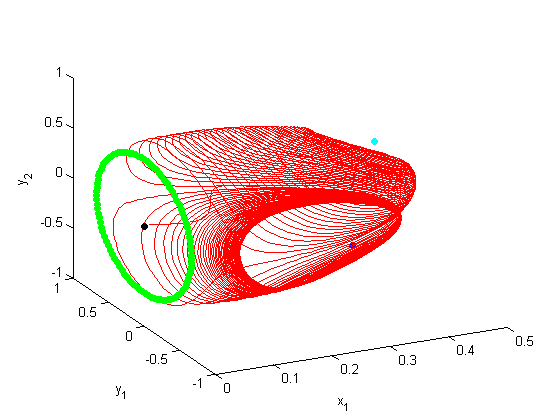
\includegraphics[width=0.35\textwidth]{kc2modesideview.png}
 (b) 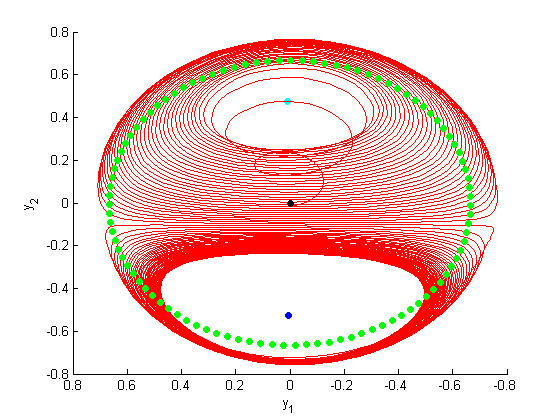
\includegraphics[width=0.35\textwidth]{kc2modedownthebarrel.png}
 (c) 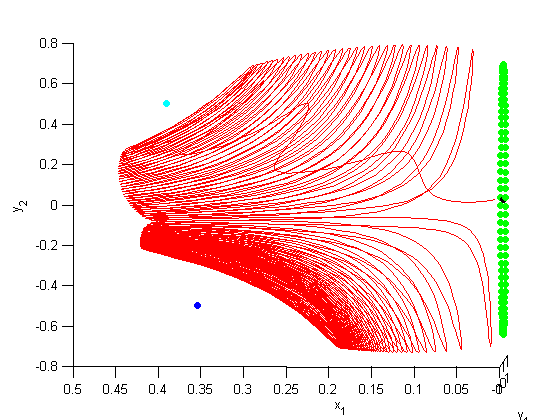
\includegraphics[width=0.35\textwidth]{kc2modeturnedview.png}
 (d) 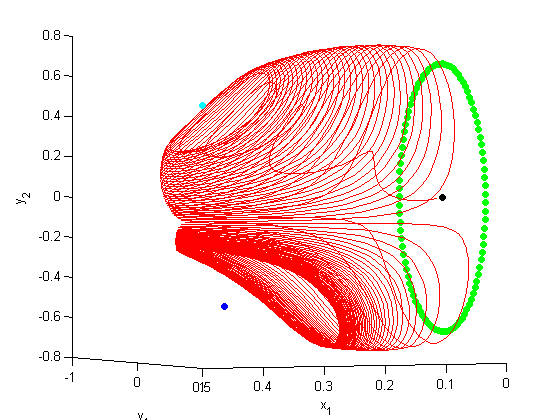
\includegraphics[width=0.35\textwidth]{kc2modelastview.png}
\caption{
(a) Symmetry reduced Hot Pants trajectory, side perspective.
(b) Symmetry reduced along the $r_1$ axis.
(c) Another perspective around one of the relative equilibrium. (d)
Perspective around the other relative equilibrium.
Finding the best angles to do this was difficult, so if you want an
interactive version, I can post it. The parameters are given as:
    $\mu_1 = 2.0 ,\, \mu_2 = 1.0,\, a_1 = -7.5,\, a_2 = -2,\, b_1 = -4,\,
       b_2 = -2.25,\, c_1 = 10,\, c_2 = -35,\, e_2 = 2$
}
\label{fig:2moderedmultieq}
\end{figure}

\item[2012-04-28 Predrag] \refFig{fig:2moderedmultieq} attractor (what is it ?) is sexy and she
knows it.

According to {\bf [2012-04-27 Daniel]},
the $[0,0,0,0]$ eigenvalues are $\lambda_1 = \mu_1$ with multiplicity 2 and
             $\lambda_3 = \mu_2 \pm i e_2$. The eigenvectors for
             $\lambda_1$ are $(1,0,0,0)$ and $(0,1,0,0)$ in the
             $(x_1,x_2,y_1,y_2)$ basis.
             The eigenvectors for
             $\lambda_2$ are $(0,0,1,0)$ and $(0,0,0,1)$
For your parameter values
             $\lambda_1 = \lambda_2= 2$,
             $\lambda_{3,4} = 1 \pm  2\,\ii$, it checks.

{\bf [Green]} $m=2$ invariant subspace: which of the eigenvalues' eigenvectors
    point into the $m=2$ world? Presumably $(-6.44444,6.88889)$.
    According to my suggestions for invariant subspaces, we would like
    repelling directions to win, which I think means $\lambda_1+\lambda_2
    >0$. If so, $(-6.44444,6.88889,-1 \pm 1.73205\ii)$ barely wins.
    However, if $\sum \lambda_j >0$ is the correct criterion, than contraction
    wins, which might be the reason that you seem to be coming closer and
    closer to the green \rpo.

{\bf [Blue]} and {\bf [Cyan]} \eqva\ might look cooler if the real part
of the expanding eigenvalue was a bit closer to zero - but maybe it does
not matter, as they rotate very fast (large imaginary parts). It could be
that because the contraction $-3.57283$ wins over the expansion $2.03058$
your attractor look like the heteroclinic connections of Armbruster,
Guckenheimer and Holmes,\rf{AGHO288}.

It's your {\bf [Green]} unreduced \rpo\ that blows wind into these Hot
Pants - green should be a point, and than these surfaces will shrink into
heteroclinic trajectories in \reducedsp?

And I really would be much happier if you used the full \statesp\ \eqva\
as templates, as is the current religion, even though it might mean
losing your Pants.  You really want a \slice\ which also reduces the
rotations within the $m_1=0$ invariant subspace.

\item[2012-04-28 Predrag] The Hot Pants do not look chaotic.  You'll have
to wade deeper. If \reffig{fig:2moderedmultieq} is in a slice hyperplane,
how wild is the full \statesp\ attractor?

\item[2012-04-28 Evangelos to Keith] \reffig{fig:2moderedmultieq} looks like a transient
to a stable limit cycle to me. You do plot $t=0$ to $t=t_{max}$, right? Why don't
you post a figure going from $t=t_{max}/2$ to $t_{max}$?

\item[2012-04-28 Keith to Evangelos]  Yes I actually did that this
morning, it turns out that it is a limit cycle.  So sadly this is not a
good situation to use.

\item[2012-04-28 Evangelos to Chaos Gang] Predrag and I do not like a
\reducedsp\ in which a relative equilibrium (such as the green orbit in
\reffig{fig:2moderedmultieq}) does not appear as a single point. I read
the explanation in [2012-04-28 Keith to Predrag] but are we sure we
don't want to symmetry reduce within invariant subspaces?
{\bf [2012-04-28 Keith]} I never intended to use this as the invariant
subspace, I just needed something to cut through the symmetries to see
what was happening instead of the full space.  I regret not having used the
insights that I gained in the chaos course.  [2012-04-29 Keith] I did not write that last sentence, but find it rather amusing.

% [ES correcting himself
% a few minutes later: I'm not the only one, Predrag is also worried. This
% blog is getting very hard to read.]

\item[2012-04-28 Predrag]
I have a really important paper to write, but doing algebra by hand is so
much easier: how to solve for \eqva\ of \refeq{PKinvEqs}? Define
\beq
A_1= \mu_1+a_1\,u+b_1\,v
    \,,\qquad
A_2 = \mu_2+a_2\,u+b_2\,v
\ee{PKinvEqs2a}
then rewrite \refeq{PKinvEqs} as
\bea
  0  &=&  2\,A_1\,u +c_1\,w
    \,,\qquad
  0  =  2\,A_2\,v +c_2\,w
\continue
  0  &=& (2\,A_1+ A_2)\,w
             +\left(c_2\,u+2\,c_1\,v\right)\,u -e_2\,q
\label{PKinvEqs3}\\
  0  &=& (2\,A_1+ A_2)\,q + e_2\,\,w
\nnu
\eea
We already know $[0,0,0,0]$ and $[0,v,0,0]$ roots, so we are looking only
for the $u>0$, $v>0$, $w,q \in \reals$ solutions; there could be problems
from the non-generic roots with either $w=0$ or $q=0$, but not both
simultaneously, syzygy \refeq{eq:syzPK} precludes that. $w$ and/or $q$
can be eliminated by rewriting \refeq{PKinvEqs3} as:
\bea
  w  &=& - \frac{2\,u}{c_1}\,A_1 = - \frac{2\,v}{c_2}\,A_2
\continue
        &\to&\quad 2\,A_1+ A_2 = - \frac{ w}{2\,u\,v}\left(c_2\,u+2\,c_1\,v\right)
\continue
  q  &=& \frac{1}{e_2}
     \left(- {w^2}/{2\,u\,v} + \,u\right)\left(c_2\,u+2\,c_1\,v\right)
\label{PKinvEqs4}\\
  w  &=& -\frac{2}{e_2} (2\,A_1+ A_2)\,q
     \,,\quad\to\quad
  q = \frac{e_2\,u\,v}{c_2\,u+2\,c_1\,v}
  \,,
\nnu
\eea
We obtain \textbf{our main result}, two (bivariate)  polynomials in two
variables $\{u,v\}$ with constant coefficients
\bea
f(u,v) &=&
  c_2\,u\,(\mu_1+a_1\,u+b_1\,v)
     -
  c_1\,v\,(\mu_2+a_2\,u+b_2\,v) = 0
\,,\qquad  deg(f) = 2
\continue
g(u,v) &=&
 \left(w^2 -  2\,u^2 v\right)\left(c_2\,u+2\,c_1\,v\right)^2
 +\,2\,e_2^2\,u^2\,v^2 = 0
\,,\qquad  deg(g) = 6
\,,
\label{PKinvEqs5}
\eea
where $w$ is to be inserted from either of the first two equations in
\refeq{PKinvEqs4}, or their average. Lots of coefficients, but we can
absorb some into rescaled quantities
$\tilde{u} = c_2\,u$,
$\tilde{v} = c_1\,v$,
$\tilde{a_1} = a_1/c_2$,
$\tilde{b_1} = b_1/c_1$,
$\tilde{a_2} = a_2/c_2$,
$\tilde{b_2} = b_2/c_1$,
and by using $A_1$ expression for $w$ factored out the pair of $u=0$
roots:
\bea
\tilde{f}(\tilde{u},\tilde{v}) &=&
  \tilde{u}\,A_1 - \tilde{v}\,A_2 = 0
\,,\qquad  deg(f) = 2
\continue
\tilde{g}(\tilde{u},\tilde{v}) &=&
 \left(2\,A_1^2
 - c_1\,\tilde{v}\right)
 \left(\tilde{u}+2\,\tilde{v}\right)^2
 +\,e_2^2\,\tilde{v}^2 = 0
\,,\qquad  deg(g) = 4
\continue
\mbox{where } &&
A_1 = \mu_1+\tilde{a_1}\,\tilde{u}+\tilde{b_1}\,\tilde{v}
\,,\qquad
A_2 = \mu_2+\tilde{a_2}\,\tilde{u}+\tilde{b_2}\,\tilde{v}
\,,
\label{PKinvEqs5a}
\eea
so we are down to 10 coefficients. Note that $e_2 \in \reals_{+}$, and if
we agree that  $\mu_1 > -\mu_2 > 0$ vi can rescale the first equation so
that in new time units $\tilde{\mu}_1 =1$, $\tilde{\mu}_2 = \mu_2/\mu_1
\in \reals_{-}$, so there are 9 coefficients in all. I see no further
rescaling simplification.

\item[2012-04-29 Predrag]
Up to a factor of 2 this equation as what Lei had as of {[2012-04-26]}
(Keith and Predrag had checked some of the algebra):
    \bea
 \frac{u^2}{c_1^2} (\mu_1 +a_1 u+b_1 v)^2
+\frac{u^2 v^2 e_2^2}{(c_2 u+2 c_1 v)^2}  &=& u^2 \, v
    \continue
\frac{u^2}{c_1^2} (\mu_1 +a_1 u+b_1 v)^2
- \frac{v^2}{c_2^2} (\mu_2 +a_2 u +b_2 v)^2 &=& 0
\,.
\label{2modefixdenom}
\eea
%\item[2012-04-26 Predrag]
Factoring the second equation one gets
\beq
\frac{u}{c_1}(\mu_1 +a_1 u +b_1 v)
\pm \frac{v}{c_2}(\mu_2 +a_2 u +b_2 v)
=0
\,,
\ee{2modeRequa4}
but we know from \refeq{PKinvEqs5} that only `-' sign is correct. The
invariant polynomials get this right and probably might cure the wrong
roots problems that [2012-04-27 Keith] has noted.  Adding, and using
\refeq{PKinvEqs4} I get
\beq
w^2 +\frac{4 u^2 v^2\,e_2^2}{(c_2 u+2 c_1 v)^2} - 4 u^2 \, v =0
\,.
\label{2modefixdenom1}
\eeq
This is {\color{red}almost} the same as the second equation of
\refeq{PKinvEqs5}? {\color{red}Please fix my algebra?}

As we already know $[0,0,0,0]$ and $[0,v,0,0]$ roots, we should divide
them out, but I do not know how to divide bivariate polynomials. Finding
roots of bivariate polynomials is not easy. As fate would have it, you can
learn all about right now:

\textbf{Sunday, April 29, 2012} --- 5:00pm --- Klaus 1116
\\
by Jason Cantarella (U Georgia),
Southeast Geometry Seminar General Audience Lecture:\\
\emph{The Square Peg Theorems or What does it mean to solve simultaneous equations?}

\begin{quote}
It's now been 101 years since Otto Toeplitz asked the simple question:
Does every closed curve in the plane with no self-intersections
contain four points which form the vertices of an inscribed square?
This talk will be an introduction for a general audience to the
various mathematical ideas which prove and generalize parts of the
square peg theorem, complete with some good pictures and animations.
The key idea for undergraduates is that the simple act of solving
a system of two equations in two unknowns (something that everyone
who took high-school math has probably done) is actually the
jumping off point for a wonderful journey into modern mathematics.
\end{quote}

At this point Google brain
\HREF{http://mathdl.maa.org/images/upload_library/22/Ford/Sturmfels907-922.pdf}
{kicks in}:

{\bf Bezout's Theorem}~~ Let $f(x, y) = g(x, y) = 0$ be a system of two
polynomial equations in two unknowns. If it has only finitely many common
complex zeros $(x, y) \in \complex^2$, then the number of those zeros is
at most $deg(f) \cdot deg(g)$.

The degree of each term in a polynomial in two variables is the sum of
the exponents, and the degree of the polynomial equals the largest such
sum. For our first equation $deg(f) = 2$, and for the second $deg(f) =
6$. So we are up to maximum 12 roots; as we know two already, we are
down to 6 roots. There is no $(u,v) \to (-u,-v)$ symmetry, so we will
have to weed out the negative $u$ or $v$ - would be nice to prove
something about the number of positive roots (the roots in the open
positive quadrant $(\reals_+)^2$) ahead of computing them.
For a single variable polynomial one has:

{\bf Descartes' Rule of Signs}~~ The number of positive real roots of a
polynomial $g(x)$ is bounded above by the number of sign alternations of
its consecutive coefficients.

For bivariate  polynomials one has to count `alternating mixed cells'.
This is an active research area of mathematics, so best to give up while
we are still ahead.

\item[2012-04-28 Bryce] The simplest root I was able to find (aside from
the obvious ones) was the following:
\beq
\left\{
   u\to   \frac{b_2 \mu_1 -b_1 \mu_2 }{a_2 b_1-a_1 b_2},
   v\to - \frac{a_2 \mu_1 -a_1 \mu_2 }{a_2 b_1-a_1 b_2},
   w\to 0,
   q\to \frac{u}{e_2 } \, (c_1 u   +  c_2 v)
\,.
\right\}
\label{invroot2}
\eeq
Haven't messed around with parameters in \refeq{invroot2} though...

\item[2012-04-29 Predrag to Bryce]
I simplified your solution, please recheck my algebra; do not
see it in \refeq{PKinvEqs5} as yet.
As $w = 2\,u |v|^{1/2} \cos \psi$, vanishing $w$ implies that $\psi =
\pi/2$. Cannot see the symmetry that would impose it. Wonder why would
that be a solution? Perhaps because of the funky $\On{2}$ symmetry
breaking $e_2$ term. As $q$ is proportional to $e_2$, there are no
solutions with $q=0$. However, \refeq{PKinvEqs5} does simplify for  $w=0$
\bea
  c_2\,u\,(\mu_1+a_1\,u+b_1\,v)
&=&
  c_1\,v\,(\mu_2+a_2\,u+b_2\,v)
\continue
  (c_2\,u+2\,c_1\,v)^2
&=&
  e_2^2\,{v}
\,,
\label{PKinvEqs6}
\eea
Both equations have  $deg(f) = 2$, so at most 4 roots, but that includes
the two we already know. The $v > 0$ case is a bit weird - a constraint
on coefficients? \(0=\mu_2+b_2\,v\), \(4 c_1^2\,v = e_2^2 \). Must have
made en error someplace...

\item[2012-04-29 Predrag] A cry in wilderness. OK, now that I've worked
out your polynomials, can you, now that you are owed by my secret skills
(OK - do not tell anybody - I looked at the articles that you cite), can
you now for once {\color{red}hear} me?

\begin{bartlett}{
It is not enough to be Hungarian, one must also have talent.
        }
\bauthor{
Paperweight on Zsa Zsa Gabor's desk
    }
\end{bartlett}

I'll be honored if you blow me off and then do the right thing, but remember
Zsa Zsa's paperweight.
Don't just screw around with zillion parameters. ChaosBook tells you to
\begin{enumerate}
  \item determine the \eqva\ (in the invariant polynomial basis), then
  \item study their stability,
  \item move parameters so that \eqva\ are nicely
        hyperbolic, \ie, on the whole they repel more than they contract.
\end{enumerate}
This way they will kick the trajectory around, not suck it in as happened
to Keith's Hot Pants or Lei's \reffig{fig:dangelmayr_proj}. You want the
repelling directions to win. If $\{\lambda_e\}$ is the set of expanding
eigenvalues, and $\{\lambda_c\}$ the set of contracting ones, I believe
you want as few expanding directions as possible (otherwise it is hard to
find the contracting directions toward the hyperbolic point, and you want
\(
\sum \lambda_e > - \sum \lambda_c >0
\,,\)
but not by very much, otherwise you never get close to the \eqv.

In particular, for the \eqv\ at the origin, pick $\mu_j$ of opposite
signs. In order to avoid the \cLe-type  near visits to the invariant
subspace (there it was the $z$ axis, here it is the $m=2$ subspace) pick
contraction within the subspace, $\mu_2 < 0$, but make it overall
repelling by making sure that $\mu_1 > -\mu_2 > 0$. {\color{red}No
parameters that you have reported so far in your experiments satisfy that.}


\item[2012-04-29 Keith]  This was what I was aiming to do for the
previous stuff, but for some reason I could only get an attractor
centered around a single \template, and not two.  Or else as I posted, I
would get a limit cycle or trajectories that converged just towards one
of the \eqva.  I will continue to toy with the parameters, but am mostly
focused on finishing up the return map stuff.

\item[2012-04-29 Keith to Predrag] How does one divide out roots
to a multinomial?  I know how to do it for a single variable polynomial,
but not a multi-variable one.  You can't use the same formalisms because
that doesn't make sense (ie I can't divide by:
$(r_1-r_{0}^{(1)})\dot(r_2-r_{0}^{(2)})$ where $r_{0}^{(1)}$ and
$r_{0}^{(2)}$ are the roots because this would imply that $r_1 =
r_{0}^{(1)}$ is always a root, and that may not be true $\forall r_2$).
I suspect one has to divide by a multinomial itself, but I do not know a
way to get this.

\item[2012-04-29 Predrag] Clipping from above [2012-04-29 Predrag]: `` I
do not know how to divide bivariate polynomials. Finding roots of
bivariate polynomials is not easy.'' It seems to be front-line research
topic in algebraic varieties that you can learn about at 5pm today.
Uurgh.

\item[2012-04-29 Daniel] Stupid AT\&T... my internet has been down. Been
working on a slightly different tangent that may \emph{perhaps} be
useful, so I'll report it. Setting the equation for $\dot{\psi}$ in the
polar form of the \twoMode\ system to zero, one can solve for
$\sin{\psi}$. Since $-1 \leq \sin{\psi}\leq 1$, one can show that any
solution must satisfy the following two conditions in $(r_1,r_2)$ space:
\beq
\dfrac{c_2}{2 c_1}r_1^2 + \left(r_2 \pm \dfrac{e_2}{4 c_1}\right)^2
  \geq \left(\dfrac{e_2}{4 c_1}\right)^2
\ee{2modeSinCond}
The $+$ condition is satisfied for any $r_1,\,r_2\,\geq 0$, but the $-$
condition is an additional constraint on what $r_1$ and $r_2$ can be.
Might prove useful if we have to brute force search for roots.

\item[2012-04-29 Predrag to Daniel] This looks promising. Repeat the
argument for invariant polynomials using \refeq{Dang86(1.2)polar}.
From \refeq{PKinvEqs4}
\bea
  q &=&  2\,u |v|^{1/2} \sin \psi = \frac{e_2\,u\,v}{c_2\,u+2\,c_1\,v}
  \,,
\label{PKinvEqs7}
\eea
and you might get similar useful bounds from the formulas for $w$.


\item[2012-04-29 Daniel to Gang] {\bf \color{red}IMPORTANT!} Updated
notation in 2mode "paper", blog, and MY matlab codes from $z_1 = x_1 + i
y_1$ and $z_2=x_2 + i y_2$ to $z_1 = x_1 + i x_2$ and $z_2 = y_1+ i y_2$
to reflect notation used in analysis of Complex Lorenz in DasBuch as per
Predrag's request. Although we've sort of moved on to $(u,v,w,q)$, I
suggest that everybody take notice and start using this notation if you
need to use 4D cartesian coordinates for anything. In fact, if you have
used the notation $z_1 = x_1 + i y_1$ and $z_2=x_2 + i y_2$ in your
codes, take 15 minutes and update it (simple find and replace works
wonders here. First, rename $y_1$ to something else, say $k$, then rename
$x_2$ to $y_1$, and finally replace $k$ with $x_2$.) so it doesn't come
back and bite us later.

\item[2012-04-29 Predrag] We are using the invariant polynomials
$\{u,v,w,q\}$ dynamics only to develop intuition, everything has to do be
done in $\pS = \{x_1,x_2,y_1,y_2\}$ and \slice\ $\pSRed$ as well. You can
see that even for the simplest conceivable $\SOn{2}$ 4-dimensional flow
one has to think about how to construct the invariant polynomial basis,
and I cannot imagine anyone could do it for high\dmn\ flows.

\item[2012-04-29 Predrag] Went to talk, told Jason Cantarella about our
bivariate polynomials. As we are interested in the positive $u,v > 0$
quadrant only, he suggest constructing vector fields from our two
polynomials, and checking the flow on $u=0$ and $v=0$ axes, and some
enclosing curve; then use Hopf index theorem to count the minimal number of
enclosed zeros.

\item[2012-04-29 Predrag] Factored out the pair of $u=0$ roots and got
our \reqv\ equations down to \refeq{PKinvEqs5a}, of degree $deg(f) \cdot
deg(g) = 2 \cdot 4$ and we are down to 9 coefficients, of which one is
positive and one is negative. {\color{red}Please check my algebra},
confirm here when done.

$g(u,v)$ and especially $f(u,v)$ in \refeq{PKinvEqs5} look pretty simple,
so I'm thinking one can simply color-code their signs (zeros are then
'nulclines'). The \eqva\ are the intersections of two sets of curves -
might be a quick way to develop an intuition about roles of various
parameters, especially if you code it as something interactive where
parameters are sliders.

\item[2012-04-29 Predrag to Bryce and Lei] Just to make command and
control structure clear: you are writing the \twoMode\
\HREF{http://www.cns.gatech.edu/~predrag/courses/PHYS-7224-12/grading.html}
{project report}. Keith is writing a separate one on return maps, and
Daniel will continue being your adviser; he will join you later in a write-up
if we use it for a publication or include it into ChaosBook. To view just
the project (without this blog) toggle the \texttt{draftfalse} switch in
siminos/cgang/setup2modes.tex.



\end{description}
